

\documentclass[nojss,article,shortnames]{jss}

\usepackage{subfigure}
\usepackage{booktabs}
\usepackage{bm}
\usepackage[latin1]{inputenc}

%\VignetteIndexEntry{Genomic prediction with the synbreed package}
%\VignetteKeywords{Genomic prediction}
%\VignettePackage{synbreed}


%%%%%%%%%%%%%%%%%%%%%%%%%%%%%%
%% declarations for jss.cls %%%%%%%%%%%%%%%%%%%%%%%%%%%%%%%%%%%%%%%%%%
%%%%%%%%%%%%%%%%%%%%%%%%%%%%%%

%% almost as usual
\author{Valentin Wimmer\\Technische Universit\"at M\"unchen 
\And 
Theresa Albrecht\\Technische Universit\"at M\"unchen 
\AND
Hans-J\"urgen Auinger\\Technische Universit\"at M\"unchen 
\And
Chris-Carolin Sch\"on\\Technische Universit\"at M\"unchen
}
\title{\pkg{synbreed}: A Framework for the Analysis of Genomic Prediction Data Using \proglang{R}}

%% for pretty printing and a nice hypersummary also set:
\Plainauthor{Valentin Wimmer, Theresa Albrecht, Hans-J\"urgen Auinger, Chris-Carolin Sch\"on } %% comma-separated
\Plaintitle{synbreed: A Framework for the Analysis of Genomic Prediction Data Using R} %% without formatting
\Shorttitle{Analysis of Genomic Prediction Data} %% a short title (if necessary)

%% an abstract and keywords
\Abstract{
High-throughput genotyping and large scale phenotyping produces massive amounts of data.
  In this vignette, we present a novel \proglang{R} package named \pkg{synbreed} for the analysis of such data to derive genome-based predictions.  It contains a collection of functions required to fit and validate genomic prediction models in  plant and animal breeding. This covers data processing, data visualization and data analysis. Thereby a versatile analysis pipeline is established within one software package. All functions are embedded within the framework of a single, unified data object. The implementation is flexible with respect to a wide range of data formats and models.  The package fills an existing gap in the availability of software for next-generation genetics research. Where necessary, the package provides gateways to other software programs to extend the field of applications.  The utility of the package is demonstrated in this document using three large-scale example data sets provided by the \code{synbreedData} R package: a simulated data set representing a maize breeding program, a publicly available mice data set and a dairy cattle data set.   
}
\Keywords{genomic prediction, quantitative genetics, pedigree-based relatedness, marker-based relatedness, data processing, visualization}
\Plainkeywords{genomic prediction, quantitative genetics, pedigree-based relatedness, marker-based relatedness, data processing, visualization} %% without formatting
%% at least one keyword must be supplied

%% publication information
%% NOTE: Typically, this can be left commented and will be filled out by the technical editor
%% \Volume{13}
%% \Issue{9}
%% \Month{September}
%% \Year{2004}
%% \Submitdate{2004-09-29}
%% \Acceptdate{2004-09-29}

%% The address of (at least) one author should be given
%% in the following format:
\Address{
  Valentin Wimmer\\
  Lehrstuhl f\"ur Pflanzenz\"uchtung \\
  Technische Universit\"at M\"unchen\\
  85354 Freising, Germany\\
  E-mail: \email{Valentin.Wimmer@wzw.tum.de}\\
  %URL: \url{http://statmath.wu-wien.ac.at/~zeileis/}
}%% It is also possible to add a telephone and fax number
%% before the e-mail in the following format:
%% Telephone: +43/1/31336-5053
%% Fax: +43/1/31336-734

%% for those who use Sweave please include the following line (with % symbols):

%% need no \usepackage{Sweave.sty}

%% end of declarations %%%%%%%%%%%%%%%%%%%%%%%%%%%%%%%%%%%%%%%%%%%%%%%



\begin{document}

%%%%%%%%%%%%%%%%%%%%%%%%%%%%%%%%%%%%%%%%%%%%%%%%%%%%%%%%%%%%%%%%%%%%%%
% Sweave
%%%%%%%%%%%%%%%%%%%%%%%%%%%%%%%%%%%%%%%%%%%%%%%%%%%%%%%%%%%%%%%%%%%%%%
%Put all in another directory
%\SweaveOpts{prefix.string=figs/article}
\setkeys{Gin}{width=0.9\textwidth}


%%%%%%%%%%%%%%%%%%%%%%%%%%%%%%%%%%%%%%%%%%%%%%%%%%%%%%%%%%%%%%%%%%%%%%
% Initial R code
%%%%%%%%%%%%%%%%%%%%%%%%%%%%%%%%%%%%%%%%%%%%%%%%%%%%%%%%%%%%%%%%%%%%%%



%% include your article here, just as usual
%% Note that you should use the \pkg{}, \proglang{} and \code{} commands.

\section[Introduction]{Introduction}
%% Note: If there is markup in \(sub)section, then it has to be escape as above.

%In the last decade, high-throughput genotyping with tens or hundreds of thousands of single nucleotide polymorphisms (SNPs) has been established for humans and many animal and plant species. With dense marker coverage, it is reasonable to assume that a large proportion of quantitative trait loci (QTL) are tagged by at least one SNP \citep{Meuwissen2001,Goddard2009a}. According to quantitative genetic theory, the observed phenotype is determined by the unobservable genetic value and the environment \citep{Falconer1996}. In agriculture, the aim is to predict the unobservable
%genotype by the phenotype and the marker profile to identify those individuals with a preferable genetic constitution.  A training set of individuals with phenotypes and marker profiles is used for parameter estimation and model training. Genetic values for the individuals in the training set are predicted from this model. This is denoted by \textit{genomic prediction}. Once the model is established, it can be used to predict the genetic value of selection candidates based on their marker profile. For the selection of individuals for the next breeding stage by the marker profile  \citet{Meuwissen2001} introduced the term \textit{genomic selection} (GS). 
%
%Developing customized algorithms was an integral part in the tool box of animal genetics researchers in the past. Nowadays, however, user-friendly software attained more attraction. Such a software is not yet available for the analysis of genomic prediction data in plant and animal breeding.  In a recent review, \citet{Heffner2009} state the urgent demand for a comprehensive software to bring GS from theory to practice. To provide a framework for the analysis of genomic prediction data, we developed a novel add-on package named \pkg{synbreed} devised for the open-source software \proglang{R}  \citep{R}. Only an open source software package is flexible enough to keep pace with advanced computational and methological challenges. Our objectives in the design of the package were (i) to provide user-friendly algorithms for non-trivial methods required in the analysis of genomic prediction data, (ii) create an analysis framework using a single, unified data object resembling a generic data structure which is suitable for a wide range of methods using genotypes and phenotypes such as GS, genome-wide association studies (GWAS) or QTL mapping, (iii) provide the methods within one open-source software package to avoid data conversion and transfer between software packages, (iv) to keep the implementation flexible with respect to the data structure for plant and animal genetics researchers, and (v) to provide a gateway to other software and \proglang{R} packages to broaden the type of possible applications. 

%Recently, GS is becoming more and more attractive. This is mainly due to three reasons. First, experimental studies confirmed an increased accuracy of predicted genetic values when using the marker data compared to models using phenotypes and pedigree only \citep{Albrecht2011}. This was already predicted from simulation studies \citep{Meuwissen2001}.  Second, generation intervals can be shortened significantly using GS because marker genotypes are available before phenotyping. In combination, the genetic gain per generation is increased substantially. Moreover, costs for genotyping are decreasing whereas phenotyping remains resource consuming. This is expected to reshape breeding programs towards the use of GS. A paradigm shift was already observed in dairy cattle breeding. Here, costs can be reduced by 92\% using GS \citep{Schaeffer2006}. 

The analysis of quantitative traits is of paramount interest in agricultural genetics. For many traits such as yield, quality or resistance against diseases and environmental stress we observe continuously distributed phenotypes. According to quantitative genetic theory, these phenotypes are determined by the joint action of many genes, the so called quantitative trait loci (QTL), and the environment \citep{Falconer1996}. To understand the inheritance of quantitative traits and to predict the unobservable genetic value of an individual are major challenges of agricultural genetics. Recently, high-throughput genotyping technology delivering tens or hundreds of thousands of single nucleotide polymorphism markers (SNPs) has become available for many crop and livestock species. The genomes of a large number of individuals can now be analyzed for their specific marker profile at high density, which allows estimating the proportion of genotype-sharing between them as well as efficient tagging of QTL in segregation analyses. In breeding, selection of the best genotypes can be conducted on high-density marker profiles once sufficiently accurate genome-based prediction models have been established. To achieve this, genomic prediction models are developed based on large training populations for which genotypic and phenotypic data are available. Once the best model is established, it can be used to predict the unobservable genetic value of selection candidates based on their marker profile. 


Research on genomic prediction (GP) will be advanced through the availability of comprehensive, user-friendly software that covers a wide range of analysis steps. In a recent review, \citet{Heffner2009} state the urgent demand for such software to bring GP from theory to practice. To provide a framework for the analysis of GP data, we developed a novel add-on package named \pkg{synbreed} devised for the open-source software \proglang{R} \citep{R}. Only an open source software package is flexible enough to keep pace with advanced computational and methodological challenges. Our objectives in the design of the package were (i) to provide user-friendly algorithms for non-trivial methods required in the analysis of GP data, (ii) create an analysis framework using a single, unified data object resembling a generic data structure which is suitable for a wide range of statistical methods employing genotypic and phenotypic data such as GP, genome-wide association studies (GWAS) or QTL mapping, (iii) provide the methods within one open-source software package to avoid data conversion and transfer between software packages, (iv) to keep the implementation flexible with respect to the data structure for plant and animal genetics, and (v) to provide a gateway to other software and \proglang{R} packages to broaden the type of possible applications.


GP uses  statistical models combining whole-genome data with phenotypic data. SNP effects are estimated from a regression of the phenotype on the marker profile. However, with a dense marker map, the model is over-parametrized. Typically, the number of SNPs $p$ exceeds the number of observations $n$. A solution is the usage of mixed models \citep{Henderson1984}. Within this framework, SNPs are used as direct predictors by modeling SNP effects or, alternatively, they are used to estimate a marker-based relationship matrix between individuals \citep{Habier2007}. The latter is used to model the variance-covariance structure for the genetic values. Recently, different models using Bayesian regression models have become popular \citep{Meuwissen2001,Campos2009}. The predictive ability of a model for GP can be assessed using an out-of sample validation. If no independent test set is available, cross-validation (CV) is used to exploit the predictive ability of a model \citep{Legarra2008,Albrecht2011}. 

Several software programs for genetics research, covering parts of the required methods, have been released within the last years.  The programs  \proglang{ASReml} \citep{Gilmour2000} and \proglang{WOMBAT} \citep{Meyer2006} provide restricted maximum likelihood (REML) estimation procedures for linear mixed models with arbitrary variance-covariance structure. The program \proglang{PLINK} implements algorithms for genome-wide association studies (GWAS) and identical-by-descent estimation. However, these programs are not stand-alone. Within \proglang{R}, different packages that tangent issues for GP are available: \pkg{qtl} for QTL analysis in experimental crosses \citep{Broman2003}, \pkg{GenABEL} for GWAS and effective SNP data storage and manipulation \citep{Aulchenko2007}, \pkg{genetics} with classes and methods for handling genetic data \citep{Warnes2003} or \pkg{BLR} \citep{Perez2010} for genome-based prediction models with Bayesian Ridge and Bayesian Lasso regression. However, there is no comprehensive program covering the specific needs of genetic researchers to analyze GP data.


In this article, we present how the \pkg{synbreed} package streamlines the analysis of GP data. The first part of the article summarizes the available data classes and functions. The second part shows by worked examples the application. The data management is guided by a single, unified data object. This forms the basis for all functions  including the coding of the marker genotypes, algorithms to impute missing genotypes and linkage disequilibrium analysis. Moreover, we provide functions to estimate coefficients of relatedness for individuals based on both pedigree or marker data. We provide several possibilities to visualize the objects generated by the \pkg{synbreed} package. We give by simulated and real data examples for the application of these functions. Mixed Models and Bayesian Regression models are used to predict genetic effects. The predictive ability of the models is compared by CV. Both model fit and validation using CV can be performed using the data object including genotypes and phenotypes directly. Finally, we give the computational requirements for the analysis steps and present possible extensions of the package.



\section[Statistical models]{Statistical models} \label{sec:statMod}

In this section, we present the statistical models used for the prediction of genetic values of individuals from a training set of individuals with phenotypes and pedigree or genotypes. We assume, that for each individual $i=1,...,n$ a single phenotypic record is available. Moreover, we consider a quantitative trait which can be modeled as being normal, i.e., $y_i = \mbox{N}(\mu + g_i,\sigma^2)$. By $\mu$, we denote the population mean and by $\sigma^2$ the residual variance.  The unobservable genetic value $g_i$ is predicted by statistical models using different data sources such as marker genotypes or pedigree. 

In the mixed model ``P-BLUP'', the genetic values are predicted using the pedigree information to construct a variance-covariance structure for the individuals. Following \citet{Henderson1984}, this model is defined by 
\begin{equation}\label{eq:animalMod}
\bf{y} = \bf{X}\bm{\beta} + \bf Z \bf a + \bf e 
\end{equation}
where $\bf y$ is the $n \times 1$ vector of phenotypic records, $\bm{\beta}$ is the vector of fixed effects and $\bf a$ is a  $n \times 1$ vector of random effects. Observations are allocated to the fixed and random effects by the  corresponding design matrices $\bf X$ and $\bf Z$. Fixed effects typically include the population mean and macro-environment  effects such as location or year. Genetic values are samples from a multivariate normal distribution
$$ \mathbf a \sim \mbox{N}( \mathbf 0, \mathbf A \sigma^2_a)$$
where $\bf A$ is the additive numerator relationship matrix and $\sigma^2_a$ the additive genetic variance \citep{Falconer1996}. The off-diagonal values of $\bf A$ are given by $2f_{i_1i_2}$ for individuals $i_1$ and $i_2$ where -- for a given pedigree -- the \textit{coefficient of coancastry} $f_{i_1i_2}$ is computed by the expected probability that two alleles are identical by descent \citep{LynchWalsh1998}. The diagonal value for individual $i_1$ is $1+F_{i_1}$ with $F_{i_1}$ being the inbreeding coefficient.  The  $n \times 1$ vector  $\bf e$ denotes the residuals with $ \mathbf e \sim N( \mathbf 0, \mathbf{I}_n \sigma^2)$ and $\mathbf{ I}_n$ is the $n$-dimensional identity matrix. Best linear unbiased estimates (BLUE) for the fixed effects $\bm{\hat{\beta}}$ and predictions for the random effects (BLUP) $\bf{\hat{a}}$ are obtained by solving the mixed model equations (MME) \citep{Henderson1984} 
$$
\left[ \begin{array}{cc}
      \mathbf{X^\top X}&\mathbf{X^\top Z}\\
      \mathbf{Z ^\top X}&\mathbf{Z ^\top Z+A^{-1}\frac{\sigma^2}{\sigma^2_a}}\end{array}\right] 
      \left[\begin{array}{c}
      \bm{\hat\beta}\\
      \mathbf{\hat a}\end{array}\right]  =
\left[\begin{array}{c}
      \mathbf{X^\top y}\\
      \mathbf{Z^\top y}\end{array}\right]
$$ 

Estimates of the variance components $\hat \sigma^2_a$ and $\hat \sigma^2$ are obtained by REML estimation. A prediction for the genetic value of individuals $i$ in the training set is given by $\hat a_i$. 
		
Genotypic data is incorporated in the mixed model ``G-BLUP''. Here, the relationship matrix based on pedigree is replaced by the genomic relationship matrix based on marker data. With the genomic relationship matrix, random deviations  from the expected relationship caused by Mendelian sampling effects \citep{Goddard2009a} can be quantified. The following equation for the genomic relationship matrix in a random mating population was proposed by \citet{Habier2007} 
\begin{equation}\label{eq:vanRaden}
\mathbf{U} = \frac{(\mathbf{W}-\mathbf{P})(\mathbf{W}-\mathbf{P})^\top}{2\sum_{j=1}^p p_j(1-p_j)}
\end{equation}
where $\bf{W}$ is the marker matrix assigning $p$ marker genotypes coded 0, 1 or 2 to $n$ individuals. $\bf{P}$ is a $n \times p$ matrix with two times the minor allele frequency $p_j$ for $j=1,...,p$ replicated  $n$ times within each column. The model ``G-BLUP'' is
\begin{equation}\label{eq:gBlup}
\bf{y} = \bf{X}\bm{\beta} + \bf Z \bf u + \bf e
\end{equation}
with 
$$ \mathbf u \sim \mbox{N}( \mathbf 0, \mathbf U \sigma^2_u)$$
where $\sigma^2_u$ is the genetic variance pertaining to model ``G-BLUP''.  The remaining parameters are defined as in model ``P-BLUP''. A prediction for the genetic value for individuals in the training set is given by $\hat u_i$. 

In the random regression model ``RR-BLUP'', the phenotype is modeled as a function of the individual SNP effects
\begin{equation}\label{eq:snpMod}
\bf{y} = \bf{X}\bm{\beta} + \bf W \bf m + \bf e
\end{equation}
where $\bf{W}$ is the $n \times p$ marker matrix and $\bf m$ the $p$-dimensional vector of SNP effects. We assume that $\bf m \sim \mbox{N}( \mathbf 0, \mathbf I \sigma^2_m) $ where $\sigma^2_m$ denotes the proportion of the genetic variance contributed by each individual SNP. A prediction for the genetic value for individuals in the training set is given by $\bf{w}_i^\top\bf{\hat{m}}$, where $\bf{w}_i$ is the $p$-dimensional vector of marker genotypes of individual $i$.  Predicted genetic values and variance components from model ``RR-BLUP'' are predictable from model ``G-BLUP'' \citep{Albrecht2011}. It is computationally advantageous to use model ``G-BLUP'' when $n<p$ because computation times are of order $O(n)$ and $O(p)$, respectively. 
%For model (\ref{eq:gBlup}), SNP effects are obtained by solving the mixed model equations from model (\ref{eq:snpMod}) using the predicted variance components from model (\ref{eq:gBlup}). The residual variance $\sigma^2$ is the same for both models.

The aforementioned models assume marker-homogeneous shrinkage of SNP effects. \citet{Meuwissen2001} suggested alternative models with marker-specific shrinkage. In this spirit, \citet{Campos2009} used Bayesian Lasso to predict SNP effects. Their model, denoted by  ``BL'', is given by 
\begin{equation}\label{eq:BayesianLasso}
\bf{y} = \bf{X}\bm{\beta} + \bf W \bf m + \bf e 
\end{equation} 
All elements but $\bf m $ are defined as in ``RR-BLUP''. The SNP effects $\bf m $ are modeled by marker-specific prior distributions
$$	\bf m \sim \mbox{N}(0,\bf T \sigma^2 ) $$
with $\mathbf{T} = \mbox{diag}(\tau_1^2,...,\tau_j^2,...,\tau_p^2)$ and the following model hierarchy
\begin{eqnarray*}	
	\tau_j^2 &\sim& \mbox{Exp}(\lambda^2),\;j=1,...,p \\
	\lambda^2 &\sim& \mbox{Ga}(\alpha,\beta) \\
	e_i &\sim& \mbox{N}(0,\sigma^2),\;i=1,...,n  \\
	\sigma^2 &\sim& \chi^{-2}(\nu,S^2)
\end{eqnarray*}
For details of the hyperparameters see \citet{Campos2009}. Parameter inference is performed within a Bayesian framework. The joint posterior distribution cannot be evaluated analytically in general. Hence Markov chain Monte Carlo (MCMC) methods are used to generate samples from the full-conditional posterior distributions. Since all full-conditional distributions are well-known distributions, a Gibbs-Sampler can be utilized to generate a Markov chain \citep{Park2008}. Prediction for the genetic value of individuals are obtained like in model ``RR-BLUP'' as $\bf{w}_i^\top\bf{\hat{m}}$.

The implementation of GP requires the prediction of the genetic performance $\mathbf{g}^* = (g_1,...,g_{n^*})^\top$ of $n^*$ unphenotyped individuals. For model ``RR-BLUP'' and ``BL'', the predicted genetic performance is given by $\hat{\mathbf{g}}^* = \mathbf{X^*}\hat{\bm{\beta}} + \mathbf{W^*}^\top\hat{\mathbf{m}}$ where $\mathbf{X^*}$ denotes the design matrix for the fixed effects and $\mathbf{W}^*$ denotes the marker matrix for the unphenotyped individuals and $\hat{\mathbf{m}}$ the prediction of the SNP effects obtained from the training set. For ``P-BLUP'', the joint relationship matrix must be defined for all individuals in the training set and the prediction set. Predictions are obtained by solving the mixed model equation for the genetic values $\bf a^*$ of the unphenotyped individuals using the estimates of the variance-components of the training set
\begin{equation}\label{eq:pred} 
\bf{y} =  \mathbf{X}{\bm{\beta}} + (\bf Z,\bf Q_0) \left(\begin{array}{l}{\bf a} \\ {\bf a^*} \end{array} \right)+ \bf e \quad \mbox{and} \quad \left(\begin{array}{l}{\bf a} \\ {\bf a^*} \end{array} \right) \sim \mbox{N}\left( \left[\begin{array}{l}0 \\ 0 \end{array}\right],\left[\begin{array}{ll} \mathbf{A} & \mathbf{A}^*   \\ {\mathbf{A}^*}^\top & \mathbf{A}^{**} \end{array}\right] \sigma^2_a \right)
\end{equation} 
with  $\bf Q_0$ being a $n \times n^*$ matrix with zeros and $\mathbf{A}$ the $n \times n$ additive numerator relationship matrix for the individuals in the training set, $\mathbf{A}^{**}$ the $n^* \times n^*$ additive numerator relationship matrix for the unphenotyped individuals and $\mathbf{A}^*$ the $n \times n^*$  additive numerator relationship matrix of the individuals in the training set with the unphenotyped individuals. Predictions for the genetic performance are obtained by $\hat{\mathbf{g}}^* = \mathbf{X}\hat{\bm{\beta}} + \bf a^*$. The same prediction scheme is employed for ``G-BLUP''. Here, the genomic relationship matrix substitutes the additive numerator relationship matrix in Equation~\ref{eq:pred} and $\sigma^2_a$ is replaced by $\sigma^2_u$.

The out-of sample performance of a GP model determines the predictive ability. Cross-validation is an assumption-free method to investigate the predictive ability of different models \citep{Legarra2008}. The data set is divided into $k$ mutually exclusive subsets, $k-1$ of them form the estimation set (ES) for model training. The $k$th subset is used as independent test set (TS) for prediction. The predictive ability of a model is the correlation $r(\mathbf{\hat{g}}_{TS},\mathbf{y}_{TS})$ of  the vector of predicted genetic values $\mathbf{\hat{g}}_{TS}$  and the vector of observed phenotypes $\mathbf{y}_{TS}$ of the individuals in the TS. Typically individuals are assigned randomly to TS and ES. However, different sampling strategies can be employed to account for population stratification. \citet{Albrecht2011} used within and across family-sampling for biparental families. The prediction bias can be assessed from a regression of the observed phenotype on the predicted genetic value \citep{Luan2009}. A regression coefficient of 1 indicates an unbiased prediction, a coefficient smaller than 1 implies inflation, a coefficient greater than 1 deflation of predicted genetic values compared to the observed phenotypes.    


	 
\section[The class gpData]{The class \code{gpData}}\label{sec:gpData}

                                      
Data for GP consists of multiple data sources. To simplify the flow and use of data, we devised a data object named \code{gpData} (``\textbf{g}enomic \textbf{p}rediction \textbf{Data}''). Any object of class \code{gpData} includes all data required for the analysis. The first step in an analysis using the \pkg{synbreed} package is to create an object of class \code{gpData}. All additional functions utilize the predefined structure. Thus, it is sufficient to create once an object with the appropriate structure and use this for further analysis. The elements are  phenotypes, genotypes and pedigree for a set of individuals. In addition, further elements for meta information on markers and individuals can be defined. The different elements are concatenated by common names for individuals and markers. They are used for data queries like in a data base. It is no prerequisite that all elements comprise the same subset of individuals or markers. Hence it is possible, e.g., to include individuals with genotypes but no phenotypes in an object of class \code{gpData}. This general structure is suitable for a wide range of data and models as employed by GP, GWAS or QTL studies. 

The advantage of a single, unified data object are manifold. When data is shared, a single data file is easier to transfer than multiple files.  By using basic summary methods, a first overview over all elements is forthcoming. Within the facilities of  \proglang{R}, an object of class \code{gpData} is stored  within the sparse binary format.  For example, the claimed storage space for the mice data, described later in this article, was reduced from 95Mb in \code{ASCII} format to 8Mb in binary format. An object of class \code{gpData} can also be used as storage for multi-year experiments. New phenotypic data can be added over years or locations. In the following sections, the different elements of an object of class \code{gpData} and their required structure are  described in more detail. 
% Furthermore, supplementary information, i.e., covariate information for individuals, can be stored within a object of class \code{gpData}. One may think of sex or age in livestock species or true breeding values in a simulation study. This data can be merged by the id with individuals in an object of class \code{gpData} and used in genomic prediction models.

%In Section~\ref{sec:functions} shows how raw data is transfered within an object of class \code{gpData} using function \code{create.gpData}.
                                                        
\subsection{Phenotypic data}

Phenotypic data is the outcome of performance tests for a set of individuals evaluating one or more traits. In plant breeding this can be the yield of a line evaluated in a field trial or in dairy cattle breeding the milk fat content measured in progeny testing. The phenotypic data are stored within the element \code{pheno}. This is an \code{array} with individuals organized in the first dimension and the traits organized in the second dimension. In case of repeated measurements for individuals, a third dimension can be used. For input, either a \code{data.frame} or a \code{array} can be used. In all cases, the phenotypic data will be converted to an \code{array}.
                                                   
\subsection{Genotypic data}

The genotypic data is stored in the element \code{geno}. This is the marker matrix with individuals organized in rows and markers in columns. In the era of SNPs, functions for data processing are limited to biallelic markers. Each entry of the marker matrix depicts the observed genotype of an individual for a marker. Marker genotypes can either be distinguished by their names (e.g., \code{"AA"}, \code{"BB"} and \code{"AB"}) or by the observed alleles (e.g., \code{"A/C","A/T",...}). 
                                                                                                                                         
\subsection{Pedigree}\label{sec:pedigree}

Pedigree information for individuals is stored in the element \code{pedigree}. The pedigree is a table of individuals of the current generation and their ancestors. The pedigree is sorted by generation, beginning with the individuals with unknown parents (coded as \code{"0"}). The content is an object of class \code{pedigree} created by the function \code{create.pedigree}.   An object of class \code{pedigree} is a \code{data.frame} with at least four variables, \code{ID}, \code{Par1}, \code{Par2}, and \code{gener}  for names of  individuals, Parent 1, i.e., sire, and Parent 2, i.e., dam, and generation, respectively. For animals, an optional variable \code{sex} can be added.                                                                                                                               

\subsection{Covariate information}

Additional information on individuals is stored in the element \code{covar}. This is a \code{data.frame} with a column \code{id} with the names of individuals that appear in \code{geno}, \code{pheno} or \code{pedigree}. Two automatically generated columns are added named \code{phenotyped} and \code{genotyped}. Both are logical and identify the individuals that are phenotyped (observations in \code{pheno}) or genotyped (observations in \code{geno}), respectively. 
%Additional information for the individuals can be added to the element \code{covar} by the user.           
                                                                                                                               
\subsection{Marker map}
                                                                 

The marker map is stored in element \code{map} of an object of class \code{gpData}. The map contains meta information about the genetic or physical positions of the marker on the genome.  More precisely, the \code{map} is a \code{data.frame} with two columns named \code{"chr"} and \code{"pos"}. The first column identifies the chromosome (\code{character} or \code{numeric}) and the second is \code{numeric} indicating the position of the marker on the genome. This can be the genetic position within the chromosomes measured in centimorgan (cM) or the physical position relative to the reference genome in base pairs. 

\subsection{Info}

Element \code{info} is used internally for additional information such as the map unit. 


Beside class \code{gpData}, several further object classes are defined within the \pkg{synbreed} package. An overview over all available classes together with their elements as well as methods and functions are given in Figure~\ref{fig:paackageDescription}. More detailed information on the functions is given in the next section.

\begin{figure}[!ht]
\centering
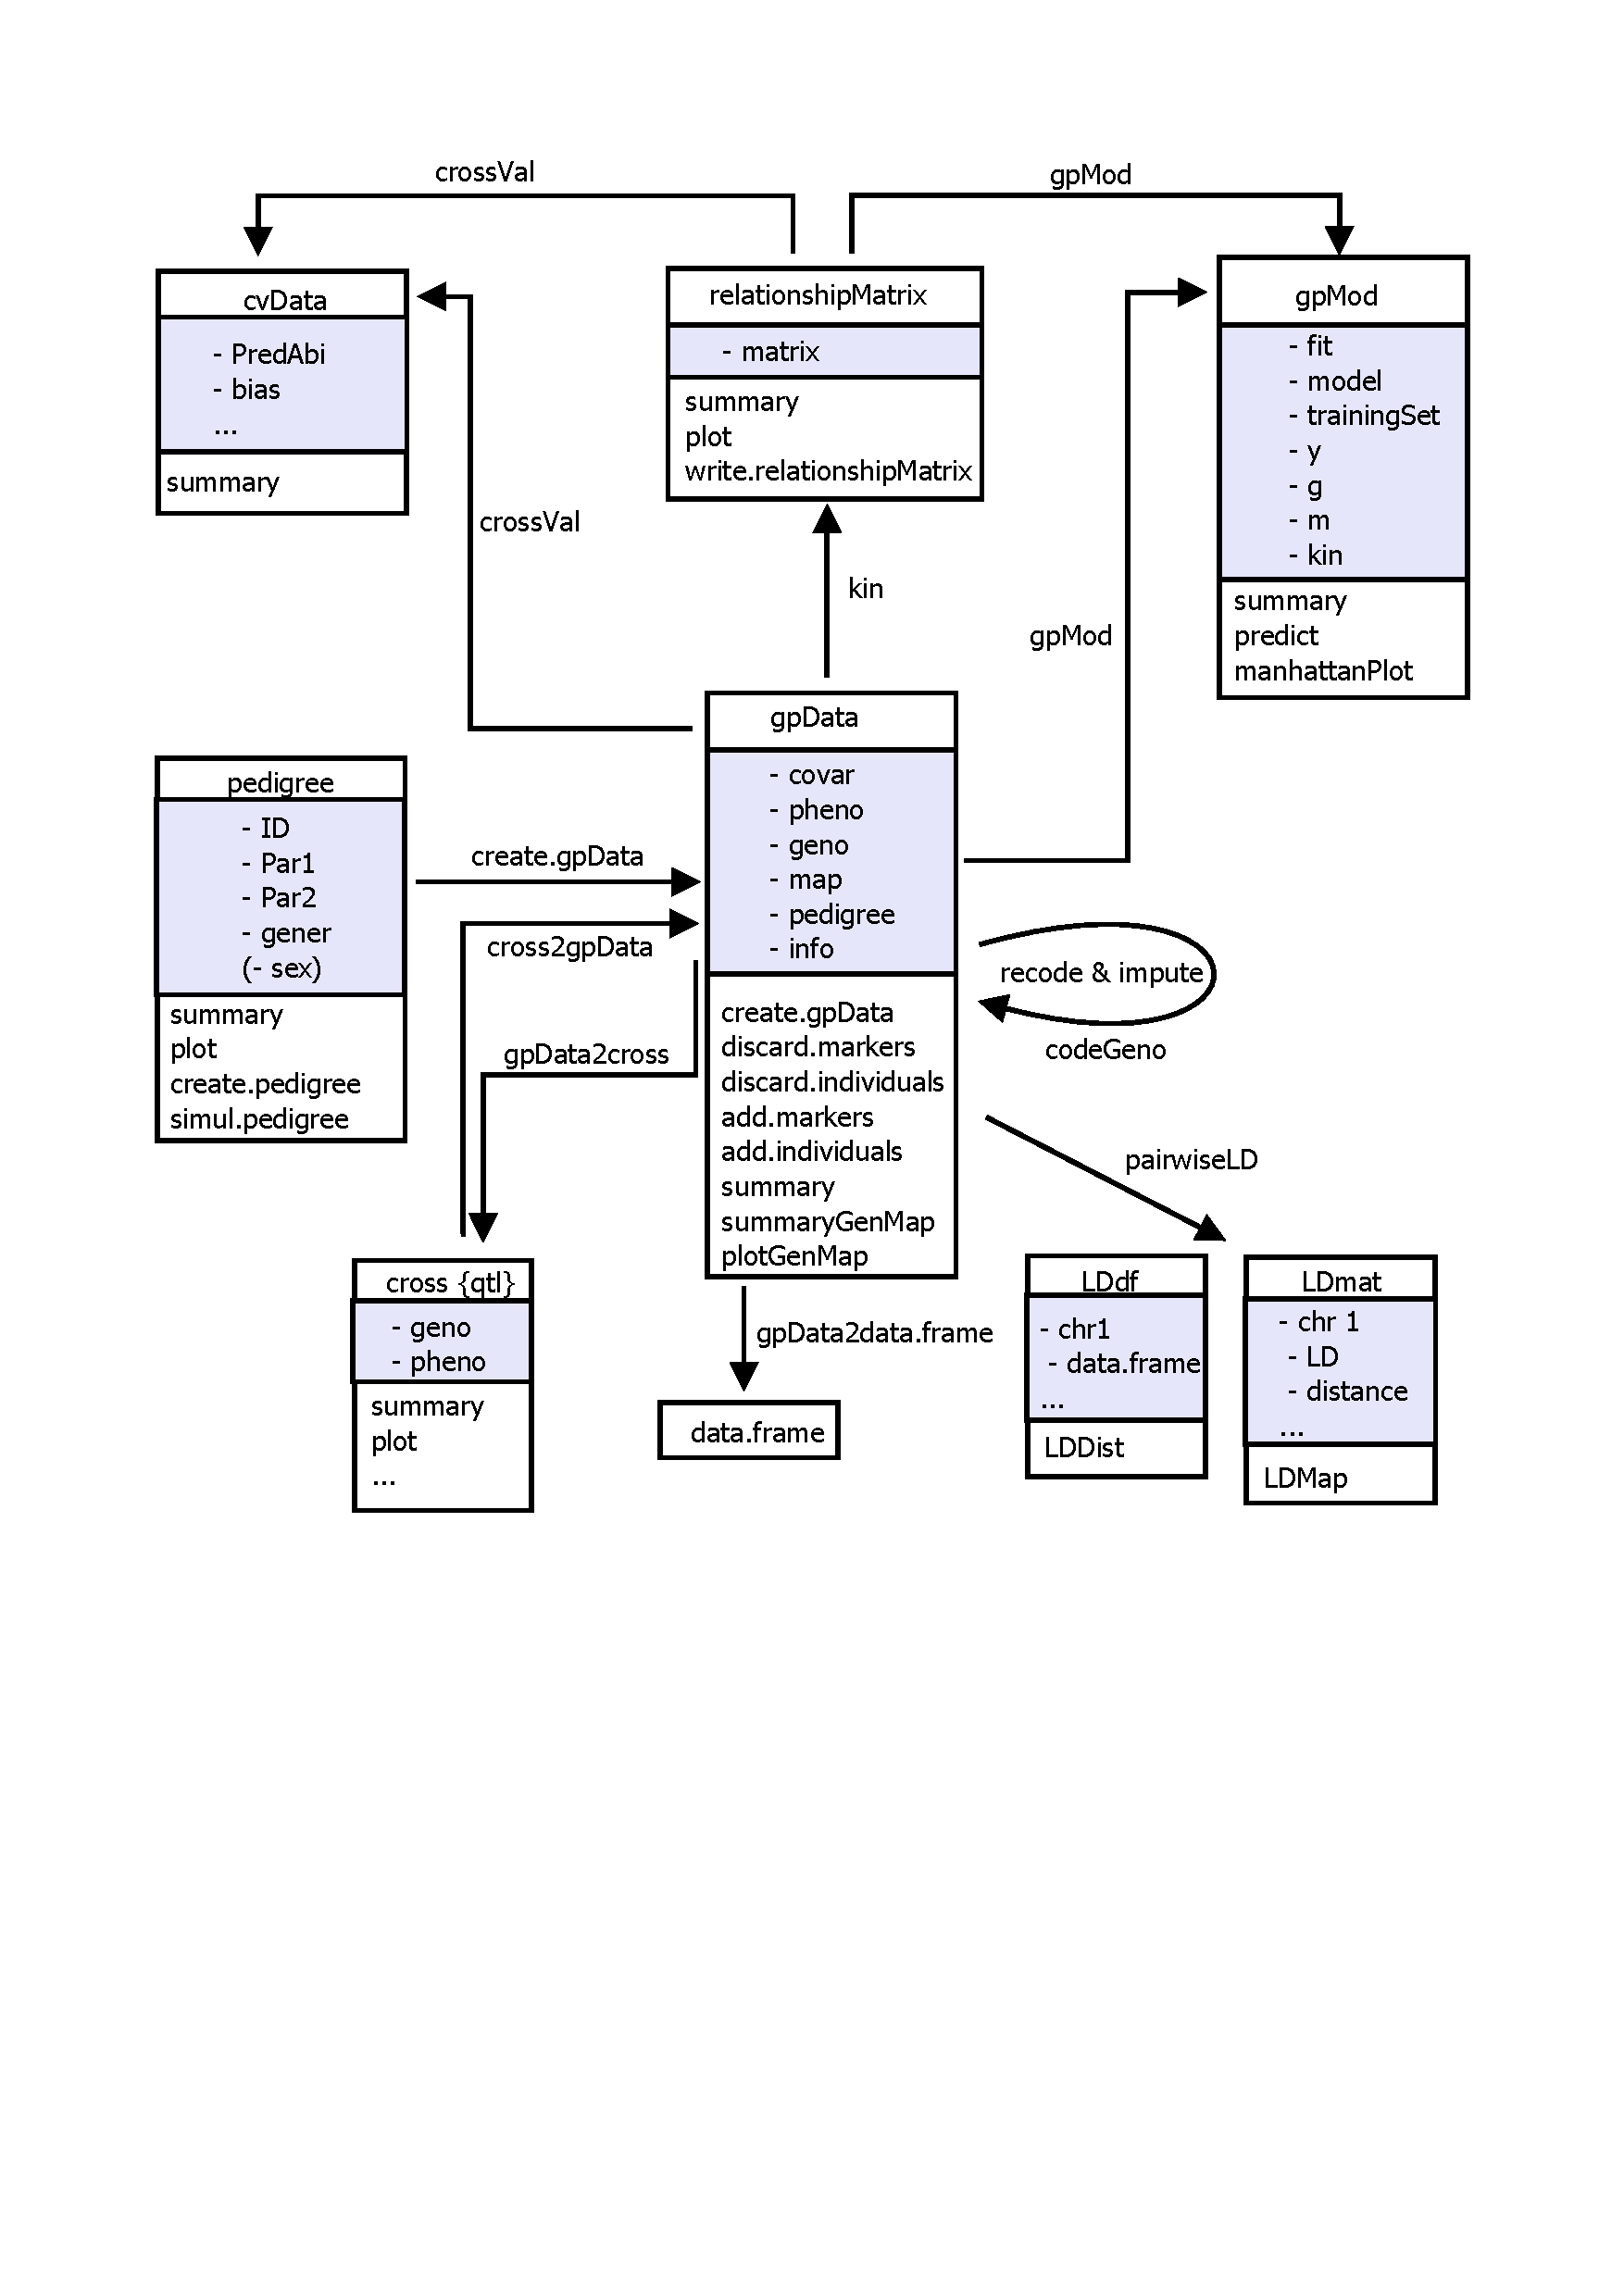
\includegraphics[trim=0cm 12cm 0cm 0cm]{figs/synbreedPackageDescription.pdf}
\caption{Overview of object classes, methods and functions within the \pkg{synbreed} package. Each box indicates a class together with the class name, the elements and the available functions and methods. The arrows indicate the data flow. The origin indicates the input argument and the head is the return value of the function.}
\label{fig:paackageDescription}
\end{figure} 

 

\section{Summary of functions}\label{sec:functions}


In this section, we present the main features of the \pkg{synbreed} package.
Their application is demonstrated by examples in Section~\ref{sec:Examples}. The preliminary step is to read-in raw data files in the workspace, e.g., using function \code{read.table}.

\subsection{Data processing}

In all analyses using the \pkg{synbreed} package, the first step is to create an object of class \code{gpData}. The function \code{create.gpData} merges the different raw data sources. The return value is a list with elements \code{covar}, \code{pheno}, \code{geno}, \code{map}, \code{pedigree} and \code{info}. The function \code{create.gpData} performs consistency checks on the data and returns an object of class \code{gpData} with the data taken from the arguments. The basic call to create an object of class \code{gpData} is
%An additional element \code{info} is appended to the object of class \code{gpData} by the function \code{create.gpData}.  
\begin{Schunk}
\begin{Sinput}
R> gp <- create.gpData(covar,pheno,geno,map,pedigree) 
\end{Sinput}
\end{Schunk}


%Pedigree information within an object of class \code{gpData} must be an object of class \code{pedigree}. The function \code{create.pedigree} creates an object of class  \code{pedigree} for a given set of individuals and their parents. The generation can be specified by the user or optional computed by the function. In the later case, generation is computed iteratively starting from the individuals with unknown parents representing generation 0 (sometimes also called ``base population") and the generation for an offspring is the maximum of the generation of either Parent 1  or Parent 2 plus 1. The resulting object of class \code{pedigree} is sorted by generation, beginning with the individuals with unknown parents.

An object of class \code{gpData} can be used as a data base with queries on individuals and markers. With function \code{discard.individuals}, a subset of individuals can be excluded from the object by removing the observations from \code{covar}, \code{pheno}, \code{geno} and \code{pedigree}. To add markers or individuals to an object of class \code{gpData}, the functions \code{add.markers} and \code{add.individuals} can be used. For subsequent analysis, other \proglang{R} packages often require a \code{data.frame} combining response variable, i.e., the trait and the marker genotypes. An object of class \code{gpData} can be converted to a \code{data.frame} using function \code{gpData2data.frame}. The function merges phenotypic and genotypic data. Multiple records for each individual result in additional rows. The \code{data.frame} can be extended by ungenotyped or unphenotyped individuals. This format applies to a variety of different functions in \proglang{R}. Moreover, we included functions for the conversion from and to class \code{cross} in package \pkg{qtl} \citep{Broman2003}, see Figure~\ref{fig:paackageDescription}.

The package \pkg{synbreed} provides several algorithms for the preprocessing of genotypic data. The algorithms are condensed in the function \code{codeGeno}. The function evaluates the following steps for the element \code{geno} within an object of class \code{gpData}.
\begin{enumerate}
    \item Discard markers that exceed a given threshold for the fraction of missing values. 
    \item Recode marker genotypes from arbitrary coding into the number of copies of the minor allele, i.e., $0$, $1$ and $2$ (see below).
    \item Impute missing values according to different algorithms (see below).
    \item Change the coding of minor and major allele whenever allele frequencies changed after step 3.
    \item Discard markers with a minor allele frequency (MAF) below a given threshold.
    \item Discard duplicated markers, retain the first copy.
\end{enumerate}                                                              

Depending on choice of arguments, not all steps are performed. A report can be printed on the screen using argument \code{verbose=TRUE}. Below, we give more details on steps 2 and 3.

\subsubsection{Step 2: Recode marker genotypes}

Genotypic data in objects of class \code{gpData} can be raw marker data or output of other software, e.g., from Illumina \code{GenomeStudio} (\url{http://www.illumina.com/software/}). Typically raw genotypic data is either coded by marker genotypes, e.g., \code{AA} and \code{BB} for the homozygous genotypes and \code{AB} for heterozygous genotypes for a locus phase or as pair of observed nucleotides, e.g., \code{A/A}, \code{A/T}, \code{G/T}, ... . The order of the alleles is not of interest in GP. Nevertheless  a common coding is required. This is in  the \pkg{synbreed} package the number of copies of the minor allele, i.e., $0$, $1$ and $2$, for a single locus. Thus, homozygous marker genotypes are coded by $0$ and $2$ and heterozygous genotypes by $1$. With this coding scheme the MAF for a marker $j$ can be computed as
$$ p_j = \frac{\sum\limits_{i=1}^n w_{ij}}{2n}\;,\;j=1,...,p$$
where $w_{ij}$ is the marker genotype for individual $i$ and marker $j$.  The heterozygous genotype must be labeled unambiguously. This can either be done by a character which clearly defines the heterozygous state (e.g., ``AB" for genotypes ``AA", ``AB" and ``BB") or a function to identify them if multiple labels declare a heterozygous genotype (e.g., first allele $\neq$ second allele for \code{A/A}, \code{A/T}, \code{G/T}, ...). With this algorithm, it is straightforward to translate every coding scheme into the number of copies of the minor allele. Some examples will be presented in Section \ref{sec:Examples}.

\subsubsection{Step 3: Imputing of missing marker genotypes}

Imputing of missing marker genotypes is often a necessary data preprocessing step. Indeed, many methods used in the analysis of GP data require a marker  matrix without missing values.  In function \code{codeGeno} missing values in the marker matrix can be replaced by one of the following algorithms (controlled by the argument \code{impute.type}):

\begin{enumerate}
          

                 
  \item Missing values are replaced using family information for fully homozygous individuals \citep{Albrecht2011}. This requires a biparental family structure with a uniform $S_0$ generation and a family size of at least $6$ individuals. In the algorithm, a missing observation $i$ for a marker $j$ in family $l$ is replaced according to the following rules: If marker $j$ is monomorphic in family $l$, the imputed value will be the observed allele. The assumption in this case is, that both parents are homozygous for the same allele. If marker $j$ is polymorphic in family $l$, the missing value is replaced from the following distribution $\Prob(x^{NA}_j=0)=\Prob(x^{NA}_j=2)=0.5$.
  
  \item The software \proglang{Beagle} \citep{Browning2009} can be used to infer missing genotypes. \proglang{Beagle} uses a Hidden Markov Model to reconstruct missing genotypes based on flanking markers. Function \code{codeGeno} creates  a directory \code{beagle} for Beagle input and output files, prepares input files and runs Beagle with default settings. The information on marker position is taken from element \code{map}. By default, three genotypes 0, 1, 2 are imputed using the allele with the highest posterior probability. This information is obtained from the \proglang{Beagle} output.   In the special case of only homozygous genotypes, values are 0 and 2 according to their ``dosage''. The dosage is the estimated number of copies of the minor allele by the \proglang{Beagle} software \citep{Browning2009}.
  
  \item A combination of the algorithms above can be used. In the first step, missing genotypes are imputed according to the family information. Here, the algorithm 1 is used for monomorphic markers and those with unknown position on the genome. In the second step, the remaining genotypes are imputed using \proglang{Beagle} as in algorithm 2.
  
    \item Missing values are sampled from the marginal allele distribution for each marker. This algorithm does not take into account data stratification. Missing values are sampled from $\{0,1,2\}$ assuming a population in Hardy-Weinberg equilibrium \citep{Falconer1996}. Thus $\Prob(x^{NA}_j=0)=(1-p_j)^2$,  $\Prob(x^{NA}_j=1)=2p_j(1-p_j)$ and $\Prob(x^{NA}_j=2)=p_j^2$. In the special case of only homozygous genotypes, a  missing value $x^{NA}_j$ for marker $j$ is replaced by a random draw from $\{0,2\}$ using the probabilities  $\Prob(x^{NA}_j=0)=1-p_j$ and  $\Prob(x^{NA}_j=2)=p_j$.
  
    \item Replacing missing values by a given value. 
\end{enumerate}

%The different imputing algorithms were compared in a simulation study. The results of the study are given in the supplementary material.
We recommend the use of \proglang{Beagle} whenever a dense marker map is available and neighboring markers can be exploited for imputation. This software package is state-of-the-art in plant and animal breeding.  However, if  information from sufficiently sized families is available, the accuracy of imputing can be increased by the usage of algorithm 3. This algorithm is also suitable for genotypic data where the marker map is sparse. 


\subsection{Data analysis}

\subsubsection{Linkage disequilibrium}

Linkage disequilibrium (LD) is defined as the non-random association of alleles at different loci. The extent of LD is determined by recombination, mutation, random drift and selection in  population history. With genotypic data, LD can be calculated as the difference between the observed and expected (assuming random distributions) allele frequencies. There are many possibilities to compute LD from genotypic data, see \citet{Foulkes2009} using the \pkg{genetics} package. In the \pkg{synbreed} package, we use the measure $r^2$ \citep{Hill1968} 
$$  r^2 = \frac{D_{vw}^2}{p_v(1-p_v)p_w(1-p_w)},$$
where $D_{vw}=p_{vw}-p_vp_w$ and $p_{vw}$, $p_v$ and $p_w$ are the frequencies of haplotype $vw$ and allele $v$ at one locus and allele $w$ at the other locus. Pairwise LD between markers on the same chromosome can be computed using function \code{pairwiseLD}. For the general case, a gateway to the software \proglang{PLINK} is established to estimate the LD. This requires that \proglang{PLINK} is available (e.g. in the working directory). A fast within-\proglang{R} solution is available for marker data with only 2 marker genotypes. The function has two different return value types: \code{matrix} and \code{data.frame}. The first is a pairwise LD matrix and the latter a list with one row for each marker pair. In both cases, results are returned chromosome-wise. Moreover, the Euclidean distance of the markers based on the \code{map} is computed. 

\subsubsection{Estimation of relatedness}

The \pkg{synbreed} package provides a unified function \code{kin} to compute pedigree-based (expected) and marker-based (realized) coefficients of relatedness. As shown in Figure~\ref{fig:paackageDescription}, coefficients are estimated for a set of individuals within an object of class \code{gpData}.  The return value is an object of class \code{relationshipMatrix}. This is a symmetric matrix with pairwise coefficients of relatedness for a set of individuals.
 
%Moreover, different types of genetic relationships such as additive and dominance can be easily extracted from the gametic relationship matrix. 
The computation of the pedigree-based relationship matrix in \pkg{synbreed} starts with the gametic relationship matrix. This approach requires only few assumptions and is very flexible with respect to special cases, i.e., homozygous inbred lines. Moreover, this computation can be extended to include two populations and dominance effects. The gametic relationship matrix is of dimension $2n \times 2n$ with $n$ being the number of individuals in the pedigree. The matrix contains the probability that two gametes are identical by descent (IBD), denoted by the equivalent symbol $\equiv$. The gametes of an individual $i_1$ are denoted by $X_1$ and $X_2$, the gametes of an individual $i_2$ are denoted by $Y_1$ and $Y_2$.  All diagonal values equal 1. The secondary diagonals contain the inbreeding coefficients $F_{i_1}=\Prob(X_2 \equiv X_1)$. Both additive and dominance relationships may be obtained from the gametic relationship matrix according to the rules in \citet{Schaeffer1989}.

Pedigree-based coefficients of relatedness include additive (argument \code{ret="add"}), dominance (argument \code{ret="dom"})  and kinship (argument \code{ret="kin"}). The additive relationship coefficient between two individuals is obtained by the sum of the four corresponding entries of the allele combinations in the gametic relationship matrix divided by $2$. The additive relatedness between individuals $i_1$ and $i_2$ is given by \citep{Bernardo2002}
$$2f_{i_1i_2} = \frac{1}{2}\left[ \Prob(X_1 \equiv Y_1) + \Prob(X_1 \equiv Y_2) + \Prob(X_2 \equiv Y_1) + \Prob(X_2 \equiv Y_2)\right].$$
The numerator relationship matrix described in Section~\ref{sec:statMod} is constructed using all pairwise coefficients $2f_{i_1i_2}$ on the off-diagonal and $1+F_{i_1}$ on the diagonal. The kinship between $i_1$ and $i_2$ is defined as $f_{i_1i_2}$. 

For non-inbred individuals, the dominance coefficients are  
$$t_{i_1i_2} = \Prob(X_1 \equiv Y_1) \cdot \Prob(X_2 \equiv Y_2) + \Prob(X_1 \equiv Y_2) \cdot \Prob(X_2 \equiv Y_1) 
.$$

If genotypic data is available, a genomic relationship can be constructed based on marker data. The matrix of genomic relationship coefficients is computed using function \code{kin} with argument \code{ret="realized"}. This requires an object of class \code{gpData} where the data in \code{geno} is coded by the number of copies of the minor allele, i.e., by using function \code{codeGeno}. The genomic relationship matrix is computed according to Equation~\ref{eq:vanRaden}. Negative values indicate pairs of individuals sharing fewer alleles than expected based on the allele frequencies and positive values indicate pairs of individuals sharing more alleles than expected from the marginal allele distributions. The denominator in Equation~\ref{eq:vanRaden} is the correction term for a random mating population \citep{Habier2007}. Corrections for other populations may be obtained by multiplying the resulting matrix by a constant. See \citet{Albrecht2011} for an example with  homozygous inbred lines.

The genomic relationship can also be computed by the simple matching coefficient \citep{Albrecht2011}. This is implemented with the argument \code{ret="sm"}, but only for homozygous inbred lines.  To account for IBS but not IBD,  \citet{Hayes2008} proposed the correction $(\mathbf{s}-s_{min})/(1-s_{min})$ where $\bf s $ is the matrix of all pairwise simple matching coefficients multiplied by $2$ and $s_{min}$ the minimum of all $\frac{n}{2}(n-1)$ values in $\bf s$  (argument \code{ret="sm-smin"} within function \code{kin}). 

Any object of class \code{relationshipMatrix} could easily be passed for further analysis to other software packages. The function \code{write.relationshipMatrix} creates a table which could be stored in an external file. Every row in the table depicts one element of the lower triangle. The table is ordered by column names within row names which is the required format for \proglang{ASReml} or by row names within column names  which is the required format for \proglang{WOMBAT}. 

\subsubsection{Statistical models}

The function \code{gpMod} provides a general interface to fit all models presented in Section~\ref{sec:statMod}. The input argument is an object of class \code{gpData}. The training set for the model are all individuals with phenotypes and genotypes (or pedigree for model ``P-BLUP'').  The mixed models ``P-BLUP'' and ``G-BLUP''  are fitted using the REML algorithm in function \code{regress} implemented in the package \pkg{regress} \citep{Clifford2009}. Model ``RR-BLUP'' is derived from model ``G-BLUP'' using the functional relationship between the models. In this case, in the first step ``G-BLUP'' is fitted and then the mixed model equations are solved for the SNP effects. The Bayesian regression models are fitted using the Gibbs-Sampler implemented in the \pkg{BLR} package \citep{Perez2010}. The variance-covariance structure in the BLUP models ``P-BLUP'' and ``G-BLUP'' is defined within the argument \code{kin} by an object of class \code{relationshipMatrix}, see Figure~\ref{fig:paackageDescription}.  The data for model training consists of all individuals with phenotypes and genotypes. All data are restricted to individuals from the training set. We include the \code{"..."} argument to allow a subtle adjustment of the model control. This includes the choice of hyper-parameters and MCMC options for ``BL''. 

For all models, the function \code{gpMod} reports the names of all individuals in the training set together with their predicted genetic performance and phenotype. For the models ``RR-BLUP'' and ``BL'' additional predicted SNP effects are returned. Moreover, the model output of the used function, i.e., \code{regress} or \code{BLR} is returned. An \code{summary} method is available for objects of class \code{gpMod}. It summarizes the number of observations in the training set and a summary for the predicted genetic performance of the individuals in the training set. Furthermore, we provide a \code{predict} method for the class \code{gpMod}. If all individuals are phenotyped, it returns the predicted genetic performance of the individuals in the training set. To predict the genetic performance of unphenotyped individuals with the models ``RR-BLUP'' or ``BL'', an object of class \code{gpData} containing the genotypic data must be passed to the \code{predict} method. To predict unphenotyped individuals with ``P-BLUP'' or ``G-BLUP'', their coefficients of relatedness must be included in the variance-covariance structure.

%matrix specified in argument \code{kin} of the function \code{gpMod}. The assortment of individuals to predict is controlled by their names in the \code{predict} method.  


\subsubsection{Cross-validation}

CV for different GP models is implemented in function \code{crossVal}. Possible models include mixed models and Bayesian regression models. To account for population stratification, different sampling strategies may be employed. Thereby in most cases the population structure will represent families or the age-group in animal breeding. The sampling strategies are
\begin{description}
	\item[random] Random sampling of the complete data set.
  \item[within popStruc] Each group is splitted into $k$ subsets to investigate within group predictive ability.
	\item[across popStruc] The ES and TS contains only complete groups for across group predictive ability.
\end{description}
The function \code{crossVal} returns an object of class \code{cvData}. This is a \code{list} of predicted genetic performance  and observed phenotypic values  for all $k\cdot r$ test sets. Moreover, the list includes individuals, size, predictive abilities and bias for each corresponding TS.

\subsection{Data summary and visualization}
                                  
In this section we present the different possibilities to visualize objects in the \pkg{synbreed} package and provide graphical or textual summaries. Thus key features of the high-dimensional objects can be assessed. For objects of class \code{gpData}, the \code{summary} method reveals general information about all elements. This includes the number of genotyped and phenotyped individuals, summary statistics (0, 25, 50, 75 and 100\% quantiles and mean) for the traits, number of markers, marker genotype frequencies and the summary for the pedigree. The \code{summary} method for an object of class \code{pedigree} includes number of individuals, parents and generations. The \code{summary} method for objects of class \code{relationshipMatrix} indicates the dimension, rank, range and number of unique values. The \code{summary} method for objects of class \code{cvData} provides information on the employed sampling scheme. Results are summarized by the minimum, mean and maximum of the predictive ability and bias across all test sets together with an estimated standard error for the mean pooled over the $k$ subsets.  
 

                         
The LD is visualized chromosome-wise.  A LD heatmap is available using function \code{LDMap}. This function is a wrapper to apply the function \code{LDheatmap} of the package \pkg{LDheatmap} \citep{Shin2006} for an object of class \code{gpData}. The LD must be organized in the \code{matrix}-format of function \code{pairwiseLD}. The function \code{LDDist} visualizes LD decay as scatterplot or stacked histogram. This requires the LD organized in the \code{data.frame} format. In the stacked histogram, the LD is visualized with bars representing fractions of SNP pairs. Breaks for the distance and LD level are controlled by the user. Moreover, a nonlinear regression curve according to \citet{Hill1988} can be added to the scatterplot. 


A \code{plot} method is available for objects of class \code{pedigree} and \code{relationshipMatrix}. The pedigree structure is visualized by a directed graph. One line is representing a generation with a vertex for each individual. Objects of class \code{relationshipMatrix} are visualized using a heatmap representation. Estimated SNP effects of an object of class \code{gpMod} can be visualized using a ``Manhattan'' plot. This is implemented in function \code{manhattanPlot}.

Genome-wide dense marker maps  require new types of visualization. The function \code{plotGenMap} provides layouts for small ($<$ 200 markers/chromosome) and high numbers of markers. In both cases, each chromosome is represented as a vertical bar. The length of the bar is given by the distance between the first and the last marker on the chromosome. For a sparse map, each marker is plotted as a horizontal bar. With a dense map, only the marker density is evaluated within equally-spaced intervals. The bandwidth for the intervals is controlled by the user. Within each interval, the number of markers is counted and visualized by a color image. In addition, function \code{summaryGenMap} returns a summary of the marker distances. This includes the number of markers, minimum, mean and maximum distances between markers by chromosome and over all chromosomes. 



       
                                   
\section{Examples}\label{sec:Examples}



\subsection{Data sets}\label{sec:dataSets}

In this section, the application of the \pkg{synbreed} package is demonstrated using the data from the \pkg{synbreedData} package. The \pkg{synbreedData} is included as a dependency in the \texttt{synbreed} package.
\subsubsection{Simulated maize data}

This simulated data resembles the output from a typical maize breeding program based on doubled haploid (DH) lines. A DH is produced by sampling gametes from heterozygous $S_0$ plants. Thus, a DH line received both gametes from a single parent and is fully homozygous. 

  Ten chromosomes of length 160 cM are simulated. True genetic values are sampled from $K=500$ segregating, biallelic QTL with equal additive effects assuming absence of dominance and epistasis
$$ g_i= \sum_{k=1}^K QTL_{ik}, \; i =1,...,n$$
where $QTL_{ik}$ is the effect of the $k$-th QTL allele for individual $i$.  Phenotypic values are simulated by adding a random environmental residual. Thus the underlying genetic model is
$$y_i=g_i+e_i, \; i =1,...,n$$
where $e_i = N(0,\sigma^2)$. Genotypic and phenotypic data was simulated for 1250 DH lines. Moreover, pedigree for additional 360 ancestor individuals is available. These ancestors can be heterozygous. The 1250 DH lines belong to 25 biparental families with 50 lines in each family. The \code{maize} data can be loaded within the \pkg{synbreed} package using
\begin{Schunk}
\begin{Sinput}
R> library("synbreed")
R> data("maize")
\end{Sinput}
\end{Schunk}
A basic overview over the contents of the \code{gpData} is available through
\begin{Schunk}
\begin{Sinput}
R> summary(maize)
\end{Sinput}
\begin{Soutput}
object of class 'gpData' 
covar 
	 No. of individuals 1610 
	         phenotyped 1250 
	          genotyped 1250 
pheno 
	 No. of traits:		   1 

     Trait      
 Min.   :120.7  
 1st Qu.:142.8  
 Median :148.9  
 Mean   :148.9  
 3rd Qu.:154.9  
 Max.   :181.8  

geno 
	 No. of markers 1117 
	 genotypes 0 1 
	 frequencies 0.339995 0.660005 
	 NA's 0.000 %
map 
	 No. of mapped markers  1117 
	 No. of chromosomes     10 

	 markers per chromosome 
	
  1   2   3   4   5   6   7   8   9  10 
 76  96  99 122  85 106 154 130 121 128 

pedigree 
Number of 
	 individuals  1610 
	 Par 1        219 
	 Par 2        221 
	 generations  15 
\end{Soutput}
\end{Schunk}

Genotypic data in element \code{geno}  comprises  1117 polymorphic SNP markers. The distribution of markers across the chromosomes is visualized in Figure~\ref{fig:maizemap} using function \code{plotGenMap(maize)}. Phenotypic data was simulated for the quantitative trait yield [dt/ha], evaluated in testcrosses of DH lines in 3 locations. Figure~\ref{fig:maizepheno} shows a histogram of average testcross performance of the 1250 DH lines.


\begin{figure}[!h]
\centering
\subfigure[Marker map]{
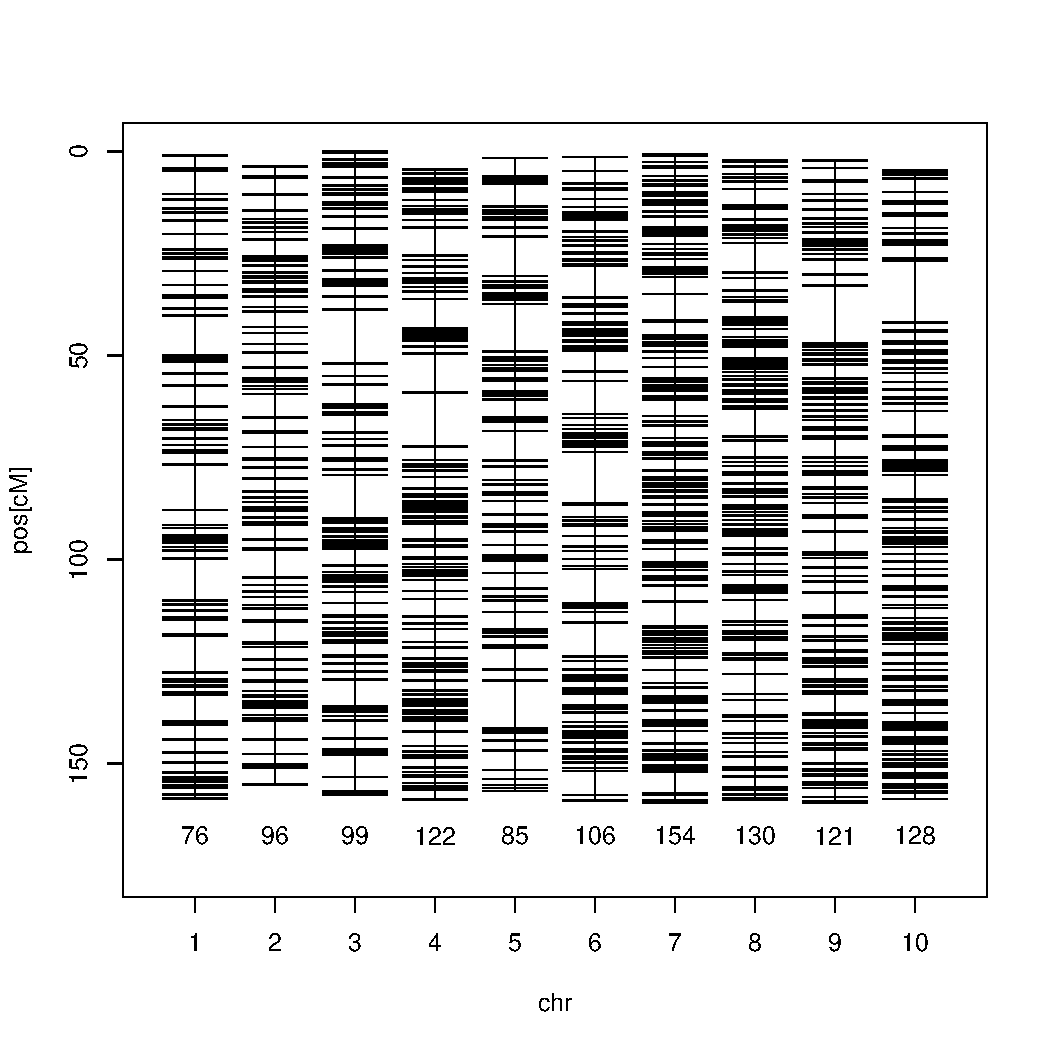
\includegraphics[width=0.45\textwidth]{figs/genMapMaize.pdf}
\label{fig:maizemap}
}\qquad
\subfigure[Phenotypic trait values]{
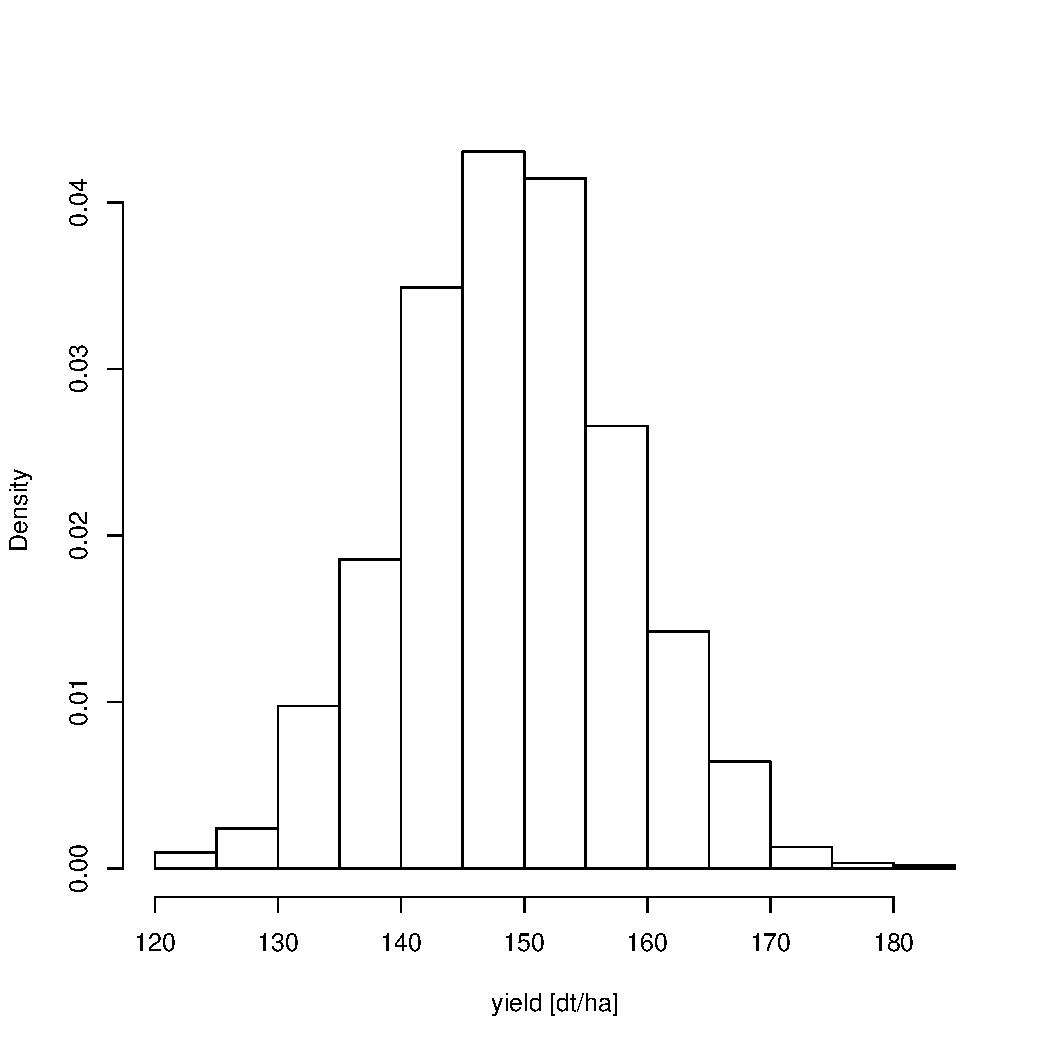
\includegraphics[width=0.45\textwidth]{figs/maizeHist.pdf}
\label{fig:maizepheno}
}
\caption{Simulated \code{maize} data with 1250 DH lines and 1117 polymorphic SNP markers. (a) Marker map with marker positions in cM and number of markers below chromosome  bars. The plot is created using \code{plotGenMap}. (b) Histogram of phenotypic trait values for testcrosses of DH lines.}
\label{fig:maizeData}
\end{figure}

\subsubsection{Mice data}

The mice data set was recently used to illustrate prospects of GP \citep{Legarra2008,Lee2010}. The data is publicly available from \url{http://gscan.well.ox.ac.uk} and comprises data of 2527 mice. They are progenies from eight inbred strains followed by 50 generations of pseudorandom mating. Original data comprises several qualitative and quantitative traits. See the website or  \citet{Valdar2006} for more details on this data set. The data can be loaded using
\begin{Schunk}
\begin{Sinput}
R> data("mice")
\end{Sinput}
\end{Schunk}
Genotypic data in element \code{geno} consists of 12545 SNP markers. Marker data is available for a subset of 1940 individuals. The marker map in element \code{map} is the sex-averaged genetic map with distances given in cM. See Figure~\ref{fig:miceMap} for a visualization of the marker map using \code{plotGenMap(mice,TRUE,FALSE,ylab="pos [cM]")}. Element \code{pheno} comprises two quantitative traits for 2527 mice: the body weight at 6 weeks age [g] and growth slope between 6 and 10 weeks age [g/day]. The distribution of both traits is shown in Figure~\ref{fig:micepheno}.  Pedigree information is not yet available from the website. The element \code{covar}  includes the variables sex (females=0, males=1), month of birth (1-12), birth year, coat color, cage density and litter.   






\begin{figure}[!h]
\centering
\subfigure[Marker map]{
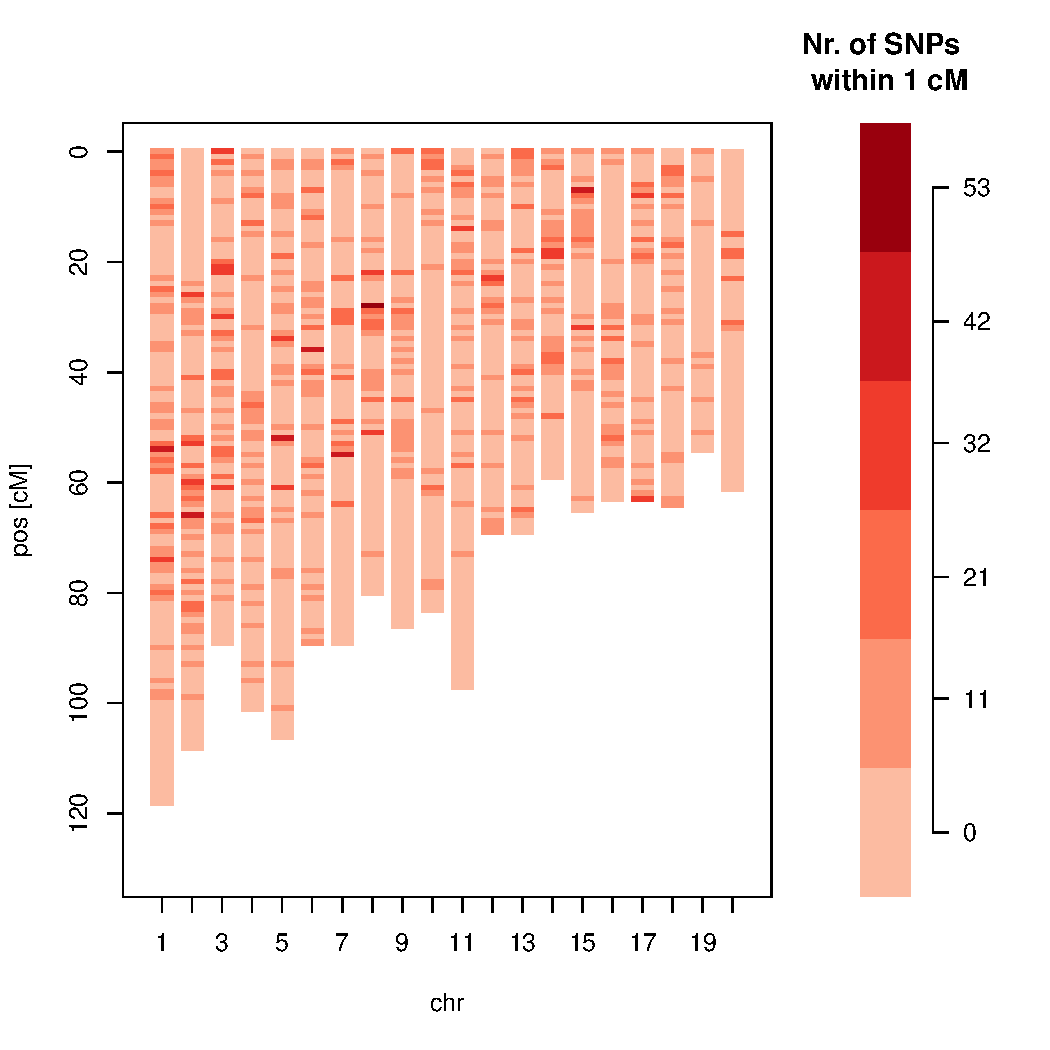
\includegraphics[width=0.46\textwidth]{figs/genMapMice.pdf}
\label{fig:miceMap}
}\qquad
\subfigure[Phenotypic trait values]{
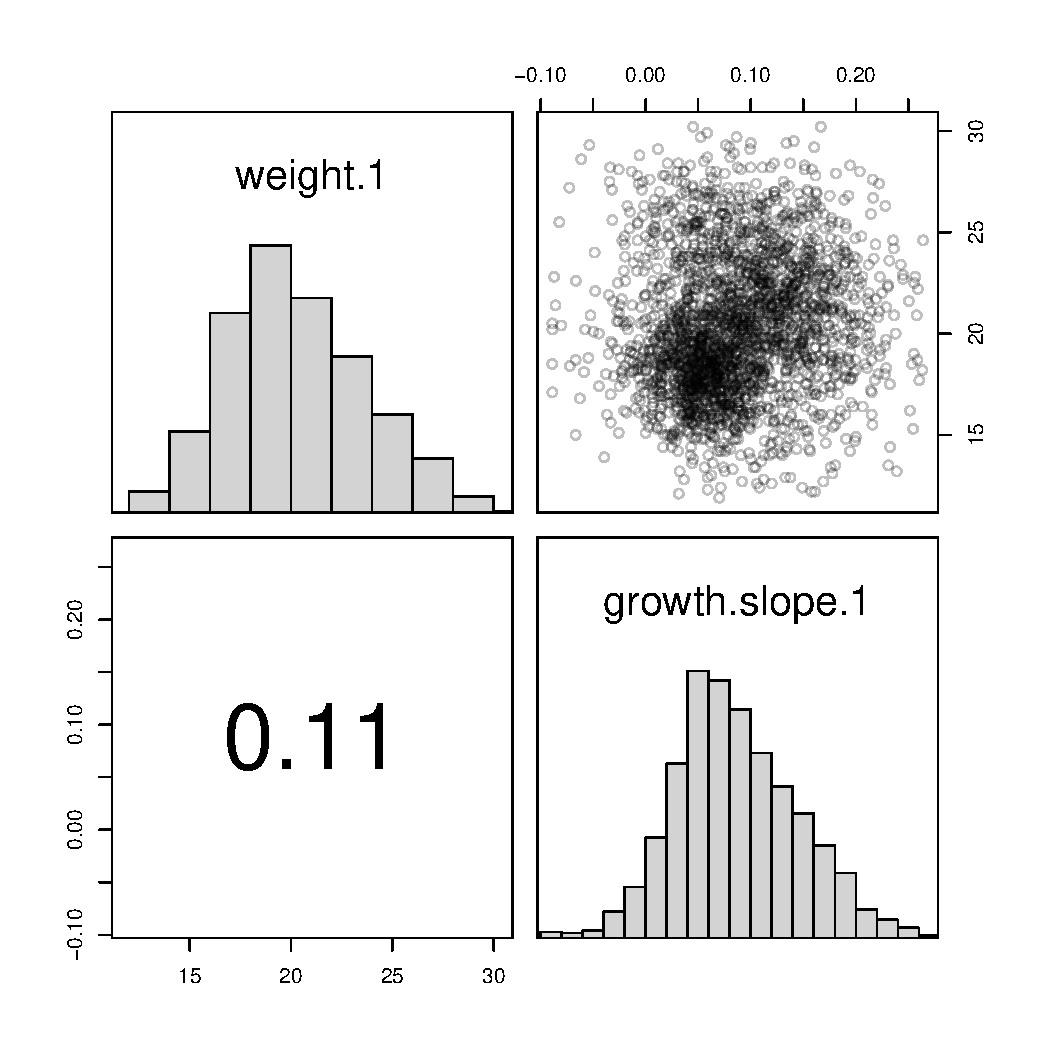
\includegraphics[width=0.44\textwidth]{figs/miceHist.pdf}
\label{fig:micepheno}
}
\caption{Publicly available \code{mice} data. (a) Visualization of the marker map comprising in total 12545 SNP markers along 19 autosomes and the X-chromosome using \code{plotGenMap}. (b) Histograms for univariate distribution of traits weight and growth slope for 2527 mice and scatterplots  for the bivariate distribution and the correlation coefficient.}
\label{fig:miceData}
\end{figure}

\subsubsection{Dairy cattle data}

This data set contains genotypic, phenotypic, map and pedigree data of 500 bulls. Genotypic and pedigree data are taken from real cattle data while phenotypes are simulated. The \code{cattle} data was provided by the Animal Breeding and Genetics group of Henner Simianer, Georg-August-Universit�t G�ttingen. The data can be loaded using
\begin{Schunk}
\begin{Sinput}
R> data("cattle")
\end{Sinput}
\end{Schunk}
Two quantitative traits are available with simulated heritabilities of 0.41 and 0.66, respectively. The distribution of both traits is shown in Figure~\ref{fig:cattlepheno}.  
Genotypic data consists of 7250 biallelic SNP markers for every phenotyped individual with missing data included. SNPs are mapped across all 29 autosomes. Distances in the SNP map are given in mega bases (Mb). See Figure~\ref{fig:cattleMap} for a visualization of the marker map using function \code{plotGenMap}. The pedigree information is available at least on parents and grandparents of the phenotyped individuals.



\begin{figure}[!h]
\centering
\subfigure[Marker map]{
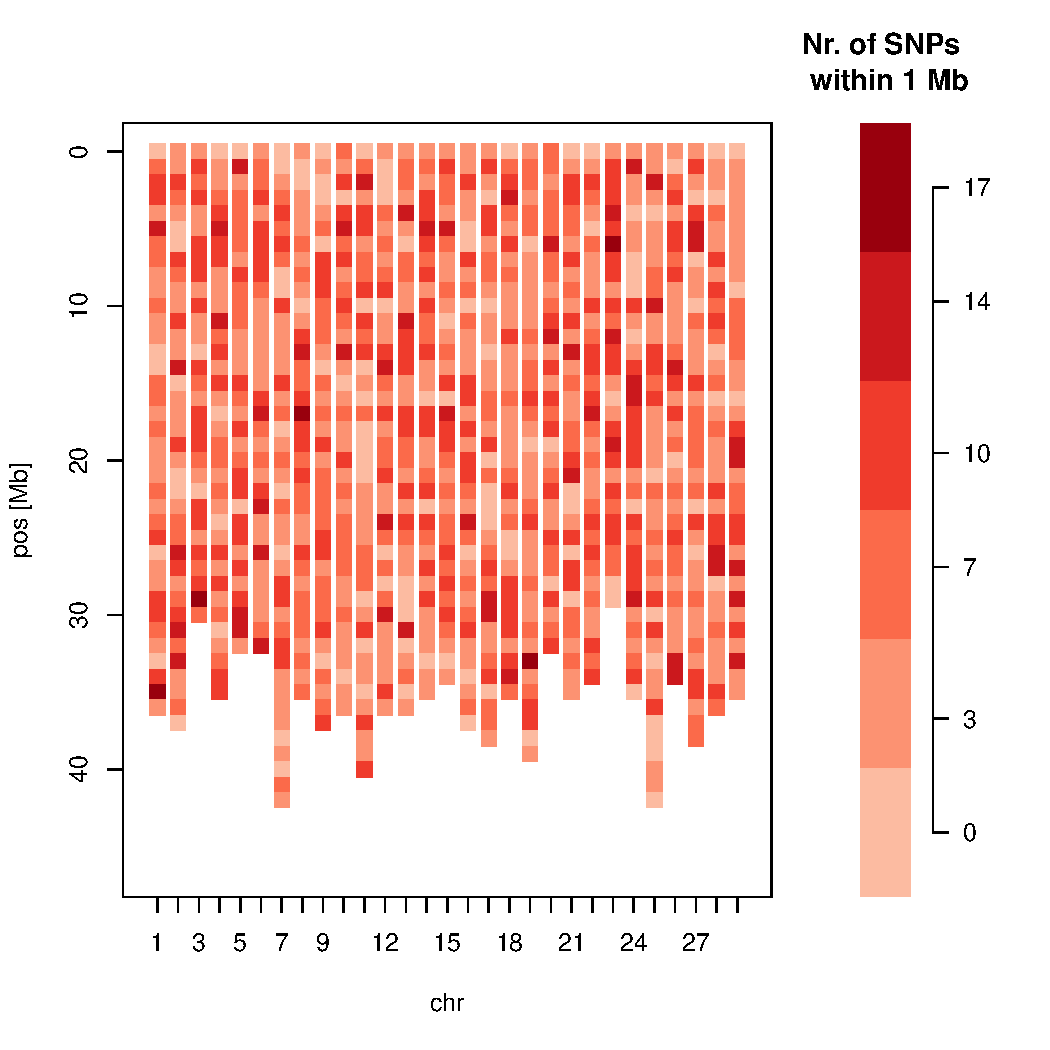
\includegraphics[width=0.46\textwidth]{figs/genMapCattle.pdf}
\label{fig:cattleMap}
}\qquad
\subfigure[Phenotypic trait values]{
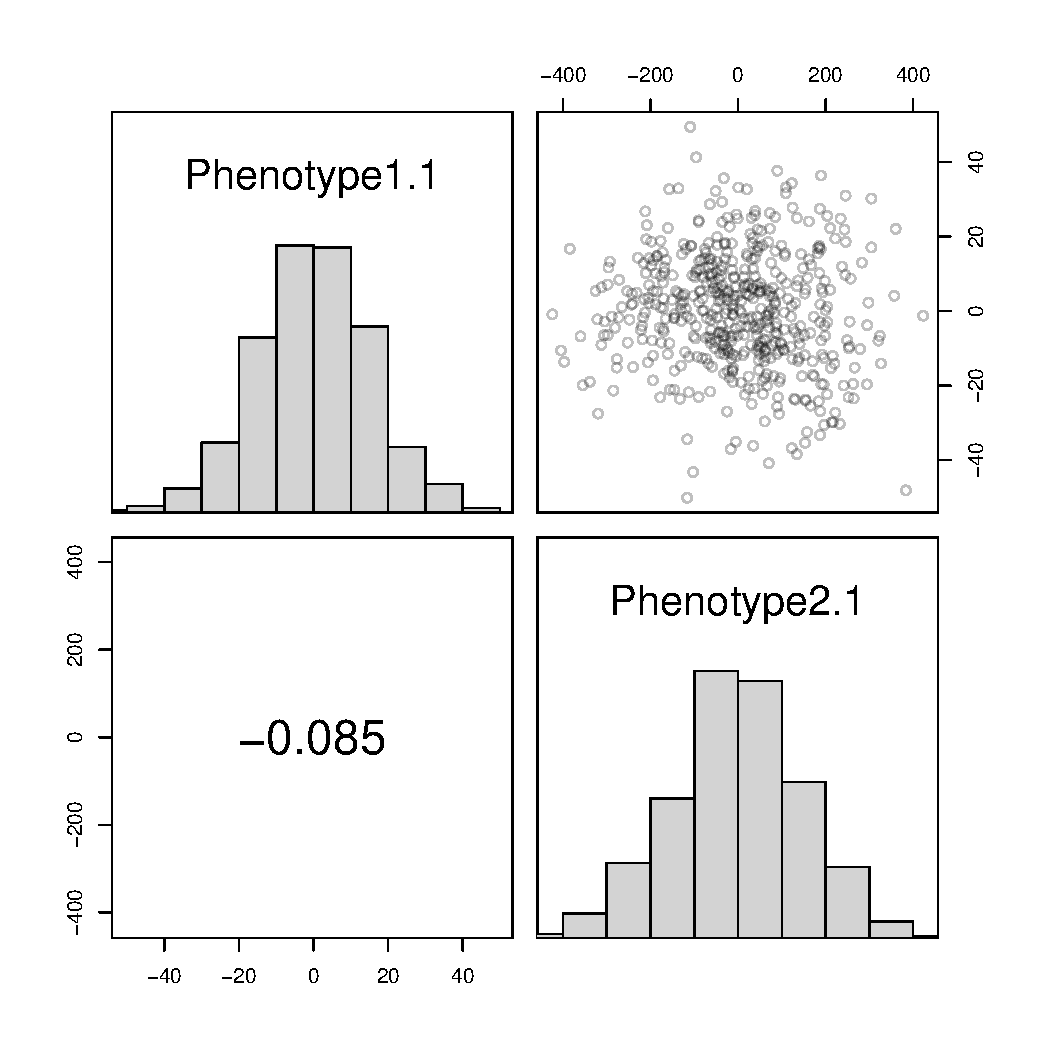
\includegraphics[width=0.44\textwidth]{figs/cattleHist.pdf}
\label{fig:cattlepheno}
}
\caption{Description of the \code{cattle} data. (a) Visualization of the marker map comprising in total 7250 SNP markers along 29 autosomes using \code{plotGenMap}. (b) Histograms for univariate distribution of traits 1 and 2 for 500 bulls and scatterplots  for the bivariate distribution and the correlation coefficient.}
\label{fig:cattleData}
\end{figure}

                                                

\subsection{Data processing and visualization}

All data sets are already given as objects of class \code{gpData}. Hence the next step is the processing of the genotypic data in element \code{geno}.  The \code{maize} data includes no missing values. Thus data processing only involves the recoding of the alleles into the number of copies of the minor allele. There are only homozygous genotypes. Hence no heterozygous genotype must be declared and genotypic data is recoded by
\begin{Schunk}
\begin{Sinput}
R> maizeC <- codeGeno(maize)
\end{Sinput}
\end{Schunk}
Resulting object \code{maizeC} is again of class \code{gpData} but with recoded genotypic data. This information is stored for further analysis as \code{codeGeno} sets \code{maizeC$info$codeGeno=TRUE}. When there are heterozygous genotypes, the argument \code{label.heter} is required. This is shown for the \code{mice} data, where genotypes are coded by the observed alleles separated by a slash symbol. A heterozygous genotype is identified whenever the first allele differs from the second allele. This can be generalized by the function
\begin{Schunk}
\begin{Sinput}
R> is.heter <- function(x) {
+      substr(x, 1, 1) != substr(x, 3, 3)
+  }
\end{Sinput}
\end{Schunk}
The function \code{is.heter} checks for unequal alleles at a locus to identify heterozygous genotypes. It is passed to the function \code{codeGeno} by the argument \code{label.heter}. 
\begin{Schunk}
\begin{Sinput}
R> miceC <- codeGeno(mice, label.heter = is.heter)
\end{Sinput}
\end{Schunk}
The function \code{codeGeno} enables a preselection of markers and the imputing of missing values. For the following analysis, we choose a threshold for the MAF of $0.05$ and of $0.01$ for the fraction of missing values. All SNPs failing these criteria  are discarded from the object of class \code{gpData}. Missing values are sampled from the marginal marker allele distribution. The corresponding call and verbose output is
\begin{Schunk}
\begin{Sinput}
R> miceC <- codeGeno(mice, label.heter = is.heter, impute = TRUE, 
+      impute.type = "random", maf = 0.05, nmiss = 0.01, verbose = TRUE)
\end{Sinput}
\end{Schunk}
\begin{Schunk}
\begin{Soutput}
step 1  : 400 marker(s) removed with > 1 % missing values 
step 2  : Recoding alleles 
step 2.1: No duplicated markers discarded 
step 3d : Random imputing of missing values 
         approximate run time  17.82  seconds 
step 4  : No recoding of alleles necessary after imputation 
step 5  : 2148 marker(s) removed with maf < 0.05 
step 6  : No duplicated markers discarded 
End      : 9997 marker(s) remain after the check

Summary of imputation 
  total number of missing values                : 23527 
  number of random imputations                  : 23527 
\end{Soutput}
\end{Schunk}
Recoding of the \code{cattle} data can be performed according to the \code{mice} data using argument \code{label.heter="AB"}.                       

In the next step, the pairwise LD for markers on chromosome 1 of \code{maize} is computed using the within-\proglang{R} solution for homozygous genotypes. We choose \code{type="data.frame"} and visualize the LD with the function \code{LDDist}.
\begin{Schunk}
\begin{Sinput}
R> maizeLD <- pairwiseLD(maizeC,chr=1,type="data.frame")
\end{Sinput}
\end{Schunk}
The LD decay for the LD data in the object \code{maizeLD} is shown in Figure~\ref{fig:LDDist}. This plot can be  generated using
\begin{Schunk}
\begin{Sinput}
R> LDDist(maizeLD,type="p",xlab="dist [cM]",pch=19,col=hsv(alpha=0.075,v=0)) 
\end{Sinput}
\end{Schunk}
for the scatterplot and                                        
\begin{Schunk}
\begin{Sinput}
R> LDDist(maizeLD,type="bars",breaks=list(dist=c(0,25,50,75,200),
+  r2=c(1,0.5,0.3,0.2,0.1,0.05,0)),xlab="dist [cM]")  
\end{Sinput}
\end{Schunk}
for the stacked histograms with user-specified breaks. The graphical layout is controlled by specifying additional graphical parameters. The LD for the recoded mice data may be obtained using the \proglang{PLINK} software invoked by the argument \code{use.plink=TRUE}.

\begin{figure}[!ht]
\centering
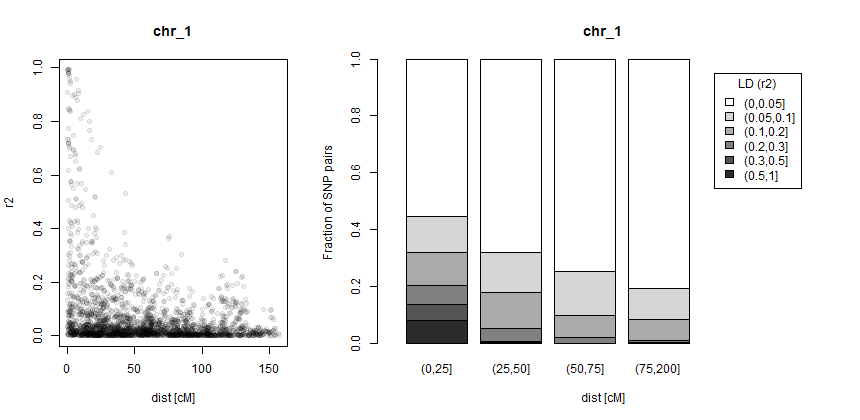
\includegraphics{figs/LDmaize.png}
\caption{LD  decay as a scatter plot (left side) and stacked histogram (right side) for 76 markers on the first chromosome for the \code{maize} data.}
\label{fig:LDDist}
\end{figure}   
                              
\subsection{Data analysis}                                                               

In the following, different coefficients of relatedness are calculated for the individuals. Pedigree-based coefficients are only inferred for the \code{maize} data. All genotyped individuals are DH lines having an inbreeding coefficient of 1. When using function \code{kin}, the special argument \code{DH} identifies DH lines in the data.  For a DH line $i_1$, $F_{i_1} = \Prob(X_1 \equiv X_2)$ is set to $1$ by the algorithm. In the \code{maize} data a variable \code{DH} in element \code{covar} indicates DH lines. The additive relationship matrix for all individuals in the pedigree is computed by
\begin{Schunk}
\begin{Sinput}
R> A <- kin(maize,ret="add",DH=maize$covar$DH)
\end{Sinput}
\end{Schunk}
The additive relationship matrix for the general case is obtained by omitting the argument \code{DH}.
A summary of the relationship matrix is obtained by
\begin{Schunk}
\begin{Sinput}
R> summary(A)
\end{Sinput}
\end{Schunk}
\begin{Schunk}
\begin{Soutput}
 dimension                    1610 x 1610 
 rank                         1460 
 range of off-diagonal values 0 -- 1.757812 
 number of unique values      1435 
 range of diagonal values     1 -- 2 
\end{Soutput}
\end{Schunk}
Genomic relationship coefficients can be computed using the recoded marker matrix. 

%Because the variance at
%individual marker loci equals  $4p_j(1-p_j)$ for homozygous inbred lines, the corresponding matrix for the \code{maize} data must be corrected with denominator $4\sum_{j=1}^p p_j(1-p_j)$ \citep{Albrecht2011}. Hence, Equation~\ref{eq:vanRaden} must be divided by 2
\begin{Schunk}
\begin{Sinput}
R> U <- kin(maizeC,ret="realized")
R> summary(U)
\end{Sinput}
\end{Schunk}
\begin{Schunk}
\begin{Soutput}
 dimension                    1250 x 1250 
 rank                         1108 
 range of off-diagonal values -0.8803719 -- 2.10971 
 number of unique values      686708 
 range of diagonal values     1.467 -- 2.964 
\end{Soutput}
\end{Schunk}
Resulting matrix \code{U} is the genome-based analogon for \code{A}. The difference in expected and realized relationship matrices can be visualized using the heatmap visualization, see Figure~\ref{fig:heatmap}. Note that only the 1250 genotyped individuals in \code{A} instead of all 1610 individuals are presented. Hence expected and realized relationship can be compared directly. The individuals were selected using the column \code{genotyped} in element \code{covar} to query only rows and columns in \code{A} for genotyped individuals.
\begin{Schunk}
\begin{Sinput}
R> plot(A[maize$covar$genotyped,maize$covar$genotyped])
R> plot(U)
\end{Sinput}
\end{Schunk}
The DH lines in the \code{maize} data are sorted by their family number. Thus the heatmap in Figure~\ref{fig:subfigHM1} is structured as $25 \times 25$ squares. Pedigree-based coefficients indicate no difference within families but differ across families. In contrast, the marker-based relationship reveals random Mendelian sampling effects within families. Thus, the heatmap provides a higher resolution for the coefficients. 

\begin{figure}[!h]
\centering
\subfigure[Pedigree-based relationship]{
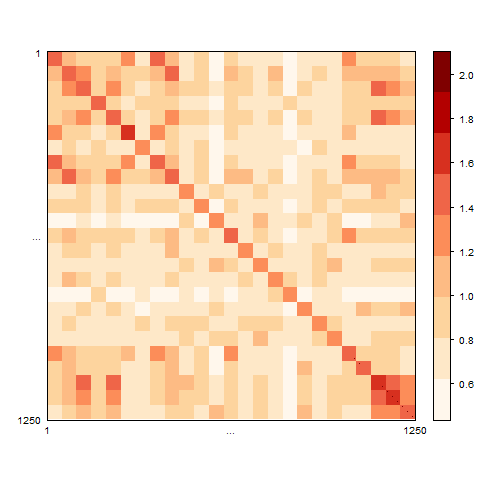
\includegraphics[width=0.45\textwidth]{figs/relMatA.png}
\label{fig:subfigHM1}
}\qquad
\subfigure[Marker-based relationship]{
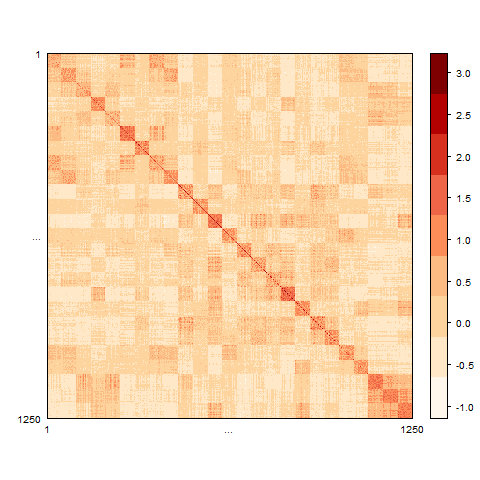
\includegraphics[width=0.45\textwidth]{figs/relMatG.png}
\label{fig:subfig2}
}
\caption{Comparison of pedigree-based (expected) relationship matrix and marker-based (realized) relationship for the 1250 genotyped individuals in \code{maize} data. Visualized are the heatmaps of pairwise relationship coefficients.}
\label{fig:heatmap}
\end{figure}

\subsection{Statistical models}

In this section, we fit statistical models to predict genetic values for the individuals in the \code{mice} and \code{maize} data. Model performance is assessed by cross-validation.

For the \code{mice} data, model ``G-BLUP'' is fitted for the trait \code{weight}. The model includes a random genetic effect and the population mean $\mu$ as fixed effect. The covariance structure for the genetic values is given by the realized relationship matrix. This is obtained by
\begin{Schunk}
\begin{Sinput}
R> UM <- kin(miceC,ret="realized")
\end{Sinput}
\end{Schunk}
The model is fitted using the function \code{gpMod}
\begin{Schunk}
\begin{Sinput}
R> miceGBLUP <- gpMod(miceC,model="BLUP",kin=UM,trait="weight")
\end{Sinput}
\end{Schunk}
The resulting object \code{miceGBLUP} is of class \code{gpMod}. A summary of the model fit is obtained by
\begin{Schunk}
\begin{Sinput}
R> summary(miceGBLUP)
\end{Sinput}
\end{Schunk}
\begin{Schunk}
\begin{Soutput}
Object of class 'gpMod' 
Model used: BLUP 
Nr. observations 1928 
Genetic performances: 
  Min.    1st Qu. Median  Mean    3rd Qu. Max    
-4.72400 -1.01600 -0.09459 -0.01184 0.96120 5.17200 
--
Model fit 
Likelihood kernel: K = (Intercept)

Maximized log likelihood with kernel K is  -3178.055 

Linear Coefficients:
             Estimate Std. Error
 (Intercept)   20.344      0.065

Variance Coefficients:
             Estimate Std. Error
       kinTS    3.704      0.498
       In       8.069      0.311
\end{Soutput}
\end{Schunk}

Estimates for the SNP effect may be obtained using ``RR-BLUP'' through 
\begin{Schunk}
\begin{Sinput}
R> miceRRBLUP <- gpMod(miceC,model="BLUP",kin=UM,trait="weight",markerEffects=TRUE)
\end{Sinput}
\end{Schunk}
Note that in this case the variance components pertaining to model (\ref{eq:snpMod}), i.e. $\sigma^2_m$ rather than $\sigma^2_u$ is reported. The model ``RR-BLUP'' uses marker-homogenous shrinkage. As a contrasting model, ``BL'' is employed which uses marker-specific shrinkage. Values for the prior distribution of $\sigma^2$ and $\lambda$ are determined using the equations of \citet{Perez2010}.
\begin{Schunk}
\begin{Sinput}
R> prior <- list(varE = list(df = 3, S = 40), lambda = list(shape = 0.8, 
+      rate = 1e-04, value = 52, type = "random"))
\end{Sinput}
\end{Schunk}
\begin{Schunk}
\begin{Sinput}
R> miceModBL  <- gpMod(miceC,model="BL",trait="weight",
+  prior=prior,nIter=12000,burnIn=2000,thin=10)
\end{Sinput}
\end{Schunk}
A summary of the model fit may be obtained using
\begin{Schunk}
\begin{Sinput}
R> summary(miceModBL)
\end{Sinput}
\end{Schunk}
\begin{Schunk}
\begin{Soutput}
Object of class 'gpMod' 
Model used: BL 
Nr. observations 2511 
Genetic performances: 
  Min.    1st Qu. Median  Mean    3rd Qu. Max    
  15.61   19.33   20.25   20.33   21.31   25.54 
--
Model fit 
MCMC options: nIter = 12000, burnIn = 2000, thin = 10
             Posterior mean 
(Intercept)  18.91775 
VarE         8.116326 
lambda       128.6805 
\end{Soutput}
\end{Schunk}

The summary reveals only marginal differences compared to the mixed model ``G-BLUP''. A ``Manhattan'' plot of the predicted marker effects is shown in Figure~\ref{fig:manhattanPlot}.

\begin{figure}[!ht]
\centering
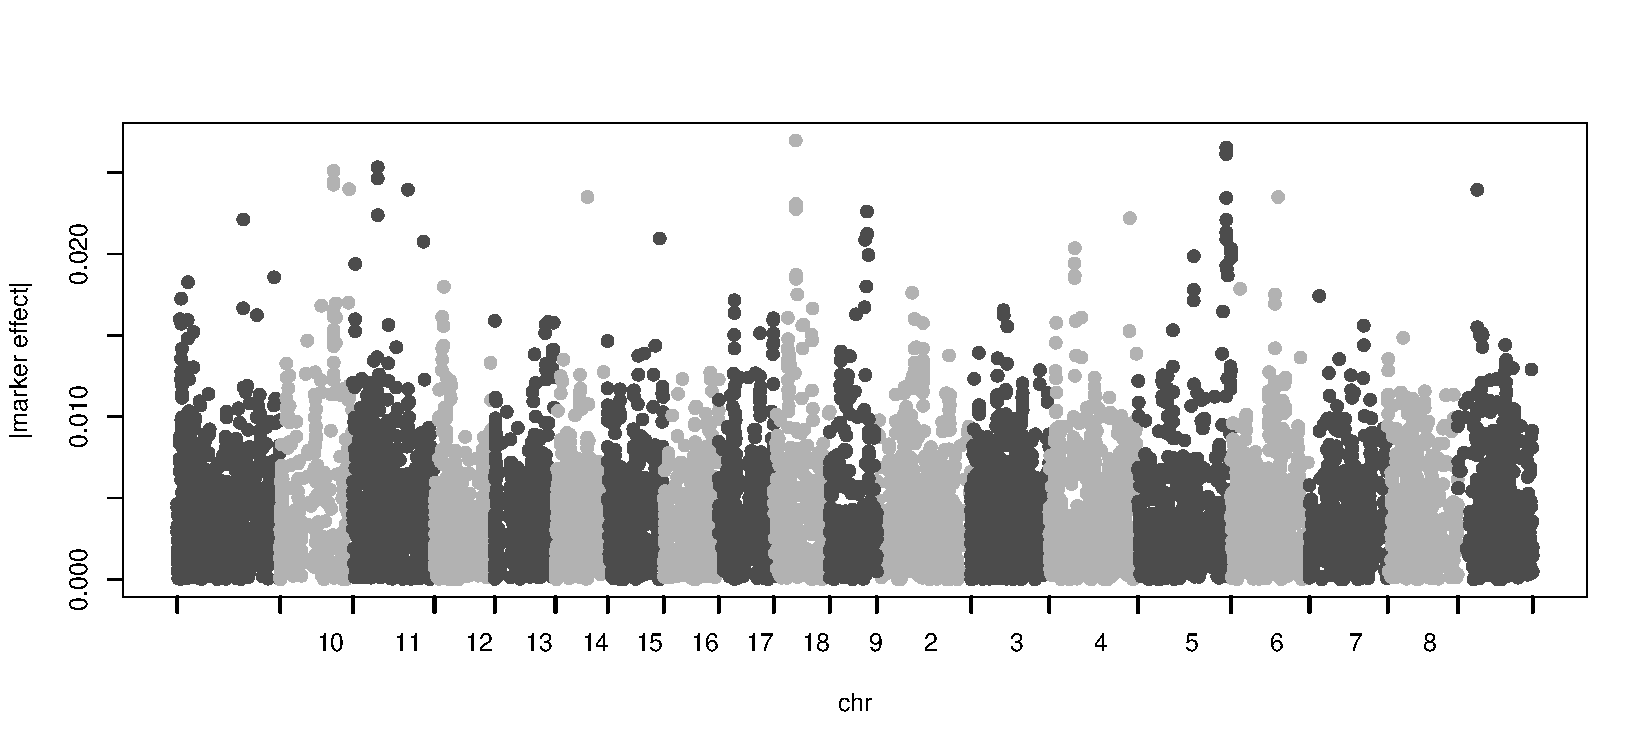
\includegraphics{figs/manhattanPlot.pdf}
\caption{Predicted SNP effects $|\hat{\bf{m}}|$ for the trait weight in \code{mice} data using ``BL''.}
\label{fig:manhattanPlot}
\end{figure}  

The estimated SNP effects of ``BL'' are used to predict the genetic performance of the 12 individuals with a missing value for weight. First, a new object of class \code{gpData} is created including the marker genotypes of the individuals of the prediction set. 
\begin{Schunk}
\begin{Sinput}
R> unphenotyped <- dimnames(mice$pheno)[[1]][is.na(mice$pheno[,1,])]
R> phenotyped <- mice$covar$id[!mice$covar$id %in% unphenotyped]
R> predSet <- discard.individuals(miceC,phenotyped)
\end{Sinput}
\end{Schunk}
Predictions for the genetic performance are obtained by
\begin{Schunk}
\begin{Sinput}
R> predict(miceModBL,predSet)
\end{Sinput}
\end{Schunk}


The predictive performance of the mixed model is judged by CV. Here, we use 2-fold CV as in \citet{Legarra2008}. The splitting into TS and ES is repeated  10 times. Individuals are assigned randomly to TS and ES. For computational ease, the variance-components are estimated once for the complete data set and committed to model training in CV. This CV scheme may be employed using
\begin{Schunk}
\begin{Sinput}
R> cv.mice <- crossVal(miceC,cov.matrix=list(UM),k=2,Rep=10,Seed=123,
+               sampling="random",varComp=miceGBLUP$fit$sigma,VC.est="commit")  
\end{Sinput}
\end{Schunk}

A summary of the CV is obtained by
\begin{Schunk}
\begin{Soutput}
Object of class 'cvData' 

 2 -fold cross validation with 10 replication(s) 
     Sampling:                 random 
     Variance components:      committed 
     Number of random effects: 1 
     Size of the TS:           964 -- 964  

Results: 
                      Min 	  Mean +- pooled SE 	  Max 
 Predictive ability:  0.2916  	  0.3697 +- 0.009471  	  0.4323 
 Bias:                0.6830  	  0.9927 +- 0.02621  	  1.2195 

Seed start:  123 
Seed replications: 
 [1] 28758 78831 40898 88302 94047  4557 52811 89242 55144 45662
\end{Soutput}
\end{Schunk}
The mean of the predictive ability is $0.37$ using random sampling. \citet{Legarra2008} reported values of $0.25$ for across family sampling and $0.67$ for within family sampling but of a different subset of the \code{mice} data. Moreover, they included a cage effect in the model. 

For the \code{maize} data, we compare the predictive ability of the pedigree-based model ``P-BLUP''  with the  genome-based models ``GBLUP'' and ``BL''.  Because phenotypic performance is evaluated as testcrosses of DH lines, the relationship matrix must be replaced by the kinship matrix \citep{Albrecht2011}. Thus, relationship matrices are divided by 2. The models are fitted by
\begin{Schunk}
\begin{Sinput}
R> PBLUP <- gpMod(maizeC, model = "BLUP", kin = A/2)
R> GBLUP <- gpMod(maizeC, model = "BLUP", kin = U/2)
R> prior <- list(varE = list(df = 3, S = 35), lambda = list(shape = 0.52, 
+      rate = 1e-04, value = 20, type = "random"))
R> modBL <- gpMod(maizeC, model = "BL", prior = prior, nIter = 6000, 
+      burnIn = 1000, thin = 5)
\end{Sinput}
\end{Schunk}

%<<echo=FALSE,results=hide>>=
%pdf("figs/mcmc_mod3Maize_lambda.pdf",width=11,height=5)
%dev.off()
%@

Convergence of the Markov chain for \code{modBL} was examined visually. No convergence problems were observed. The model performance is measured by the predictive ability $r(\mathbf{\hat{g}}_{TS},\mathbf{y}_{TS})$ from CV. The accuracy is defined as the correlation of the predicted genetic value with true breeding values $r(\mathbf{g},\hat \mathbf{g})$ for the whole data set. We use 5-fold CV with 10 replications. The results are summarized in Table~\ref{tab:resMaizeMod}. The models using marker data outperform the pedigree-based model ``P-BLUP''. However, the average predictive ability of ``BL'' using  marker-specific shrinkage is similar compared to ``G-BLUP'' using marker-homogeneous shrinkage. 



\begin{table}[h]
\centering
\begin{tabular}{llll}
\toprule
Model & \multicolumn{2}{c}{cross-validation}  & $r(\mathbf{g},\hat \mathbf{g})$ \\
&  $\bar{r}(\mathbf{\hat{g}}_{TS},\mathbf{y}_{TS})$ (s.e.) & avg. bias (s.e.) &  \\
\midrule
P-BLUP & 0.22 (0.002) & 1.00 (0.013) &0.587  \\
G-BLUP & 0.53 (0.002) & 1.00 (0.007) &0.856  \\
BL & 0.53 (0.002) & 1.01 (0.006) & 0.856  \\
\bottomrule
\end{tabular}
\caption{Comparison of the model performance of pedigree-based mixed model ``P-BLUP'', marker-based mixed model ``G-BLUP'', and Bayesian Lasso regression ``BL'' with respect to the predictive ability, the prediction bias and the accuracy.}
\label{tab:resMaizeMod}
\end{table}

\subsection{Computation times}
% from file compTimes.R

A crucial point in GP are computation times. In this section, we evaluate the computational requirement for the algorithms implemented within the \pkg{synbreed} package. The scaling with respect to the number of data points can be roughly assessed by a comparison of the \code{maize} and \code{mice} data. The number of data points in the marker matrices are $1250\cdot1117\approx1.4\cdot10^7$ and $1940\cdot12545\approx2.4\cdot10^8$, respectively. We list in Table~\ref{tab:compTimes} the elapsed system times on a standard PC (Intel Core 2, 2.8 Ghz, 4 GB RAM). To impute with the \code{maize} data, a fraction of $0.444$\% of the marker genotypes was masked. This corresponds to the number of missing data points in the marker matrix of the \code{mice} data.


\begin{table}[h]
\centering
\small
\begin{tabular}{llrr}
\toprule
& & \multicolumn{2}{c}{Computation Times [sec]} \\
Analysis step & Function & \code{maize} data & \code{mice} data \\
\midrule
Load data & \code{load} & 0.6  & 9.4 \\
Summary & \code{summary.gpData} & 3.0  & 6.2  \\
Plot marker map & \code{plotGenMap} & 0.4  & 0.2  \\
Recoding genotypes & \code{codeGeno} & 5.8 & 68.3  \\
Imputing genotypes (\code{"random"}) & \code{codeGeno} & 5.9$^a$  & 71.9  \\
Imputing genotypes (\code{"Beagle"}) & \code{codeGeno} & 67.0$^a$  & 2695.8  \\ 
Imputing genotypes (\code{"family"}) & \code{codeGeno} & 9.0$^a$  & NA  \\ 
Imputing genotypes (\code{"beagleAfterFamily"}) & \code{codeGeno} & 67.26$^a$ &  NA \\ 
Pairwise LD (only Chr. 1) & \code{pairwiseLD(,chr=1)} & 2.4  & 679.7  \\ 
Pedigree-based relationship & \code{kin(,ret="add")} & 137.8 & NA \\ 
Marker-based relationship & \code{kin(,ret="realized")} & 1.2  & 47.2 \\ 
%1 $\times$ 5-fold CV (given var. comp.)& \code{crossVal} &  &     \\ 
%1 $\times$ 5-fold CV with Bayesian Lasso$^b$& \code{crossVal} &  &     \\ 
\bottomrule
\end{tabular}
\caption{Elapsed system times (seconds) for the analysis steps using the \pkg{synbreed} package. $^a$ after randomly masking $0.444$\% values, NA=computation not possible because no pedigree is available.}
\label{tab:compTimes}
\end{table}

We observed, that the computation times for many algorithms scale linearly with the number of data points. For a $50$k SNP chip and $1000$ individuals the recoding of the alleles is performed in less than 5 minutes on a standard PC. The marker-based matrix is  computed within the same time frame. The model ``G-BLUP'' can be fitted in less than a minute. Hence, predictions for the genetic value are available in only a few minutes. However, additional analysis steps such as CV - depending on the number of splits and replications - are computationally intensive. Imputing of missing values using \proglang{Beagle} is very accurate but slow for a dense  genome-wide marker map. For a family-stratified population of homozygous inbred lines the \code{"family"} algorithm is a faster alternative.


\section{Conclusions and future work}\label{sec:outlook}


% data base
The package \pkg{synbreed} provides a valuable tool within the plant and animal genetics researchers software toolbox. It offers a comprehensive collection of methods required in the analysis of GP data. The data flow is guided by a single, unified data object. Once an object of class \code{gpData} is created, all analysis steps rely on its structure.  Moreover,  it is very convenient to share objects of class \code{gpData}. A key issue is the generality of the class \code{gpData}. We minimized the requirements concerning the data structure. This includes replicated and unreplicated trials for phenotypic data as well as arbitrary coding of marker data either by alleles or marker genotypes. Consequently, the package can also be applied in GWAS or QTL studies. For the latter, we included a gateway to the package \pkg{qtl}. The \pkg{synbreed} package is implemented as generic as possible. Hence, the package is suitable for both plant and animal genetics researchers and not limited to any species. We have successfully tested this framework for the analysis of several scenarios with simulated and experimental data from different  species (maize, rye, dairy cattlen, rice and Arabidopsis). 
%In future, an example data set based on experimental data from dairy cattle will be included in the package. 

Next generation genetics research involves computer-intensive methods to analyze massive amounts of high-throughput genotyping and large scale phenotyping data. Especially in the plant breeding community, there is a strong demand for robust standard software. We designed this package to provide access to standard methods required in GP. The \pkg{synbreed} package provides an interface to fit robust standard parametric GP models being publicly available. This allows researchers to conduct standard analyses, e.g., using mixed models. Moreover, the framework of \proglang{R} enhances the analysis and visualization of results in one software. All code is given in the \proglang{R} language. This permits the users to customize the methods to specific needs. When necessary, we provide gateways to standard software such as \proglang{Beagle} or \proglang{Plink}. Beside research and routine analysis, the package is also useful in the education of young scientists and breeders. It provides fast access to a wide range of different analysis methods and a hand-on tutorial with example data sets. Most functions have default values and short argument lists. Thus graduate students can gain expeditious insight into the statistical models and apply GP methods without having profound programing skills.


One objective of the \pkg{synbreed} package was to create a gateway to related software programs. Thereby we utilize the strength of \proglang{R} to integrate functions by the package structure. We provide an interface to fit GP models using the mixed and Bayesian regression models. The model performance can be investigated using cross-validation.  The function \code{gpData2data.frame} allows the conversion to a \code{data.frame}. This comprehensive format can be used by many other \proglang{R} functions. Other software packages such as \proglang{ASReml}  or \proglang{WOMBAT} are frequently used in genetics and breeding research. An object of class \code{relationship} matrix can be stored as a file using function \code{write.relationshipMatrix} which meets the required formats for \proglang{ASReml} or \proglang{WOMBAT}. Thus data in \pkg{synbreed} package can be used straightforward by other software. Moreover, we included functions to prepare the input files for the programs \proglang{Beagle} and \code{Plink}. We provide an interface to use the methods therein for objects of class \code{gpData}. Combining the functionality of \proglang{R} with \code{Sweave} \citep{Leisch2002} and \LaTeX \, enables to create automatic reports  presenting results for e.g., predicted genetic performance and SNP effects within tables and graphics.
This is a step towards automatized analysis pipelines in the analysis of next generation genotype and phenotype data.
% automatic reports
%The \pkg{synbreed} package provides a framework for the analysis of genomic prediction data within the 
%environment for statistical computing \proglang{R}. Combining the functionality of \proglang{R}
%with \code{Sweave} \citep{Leisch2002} and \LaTeX \, enables to create automatic reports  presenting results for e.g., predicted %breeding values and variance components together with tables and graphics. This will be especially valuable  as required time and effort is significantly reduced for a routine analysis of big field trials and the evaluation of a series of simulated data sets. Here, usually multiple data sets must be generated and analyzed to compare different scenarios. This document is available in \pkg{synbreed} as a package vignette and thus this \code{Sweave} code may serve as a layout for such automatic reports. 

There is no universal constraint in the \pkg{synbreed} package with respect to the number of data points. Rather computational facilities impose limitations.  Table~\ref{tab:compTimes} gives an overview of computation times for both data sets. Various analysis steps are performed in seconds. In general, the elapsed time increases linearly with respect to the number of data points. However, as data output from next generation sequence technology is emerging faster than computational capacities, additional effort is required to improve the algorithms. The open-source structure of \proglang{R} allows the user to customize the algorithms. Solutions can be the use of parallel computing utilizing the power of multi-core systems \citep{Schmidberger2009}. Hence, computation times are likely to be reduced by an order of magnitude, especially on a multi-core cluster. The claimed workspace can be reduced by using sparse matrix methods (e.g., \proglang{R} package \pkg{ff}, \citet{Adler2010}). The current version of the package enables genotype-based analyses. However, using haplotypes is desirable, too. For the future, we are aiming to include an additional data object for haplotyes and provide tools to analyze them. As available amount of data points are expected to increase, future work will also include the embedding of foreign languages, i.e., \proglang{C}. 

\section*{Acknowledgments}

This research was funded by the German Federal Ministry of Education and                                                     
Research (BMBF) within the AgroClustEr \textit{Synbreed} $-$  \textit{Synergistic plant and
animal breeding (FKZ 0315528A)}. We gratefully acknowledge Larry Schaeffer for providing us \proglang{R} code which is used by functions \code{kin} and \code{MME}, Michael H�hle for valuable discussions with respect to the manuscript and package design and Richard Mott for his help with the \code{mice} data. Henner Simianer, Malena Erbe and Christian Reimer are acknowledged for providing and preparing the \code{cattle} data. All users of the beta-version of the \pkg{synbreed} package are acknowledged for their suggestions and contributions. 
%Valentin Wimmer gratefully acknowledges the support by the Faculty Graduate Center Weihenstephan of TUM Graduate School at Technische Universit�t M�nchen, Germany.



%\bibliographystyle{jss}
\bibliography{IntroSyn}

\end{document}
